\documentclass{article}
\usepackage[utf8]{inputenc}
\usepackage{amsmath}
\usepackage{fancyhdr}
\usepackage{natbib}
\usepackage{graphicx}
\usepackage{systeme}
\usepackage{enumitem}
\usepackage{hyperref}
\usepackage{graphicx}
\graphicspath{ {./visuals/} }


\title{\LARGE EmbedUR Internship Final Report}
\author{\Large Siddharth Nath}
\date{\Large August 2021}

\pagestyle{fancy}
\fancyhf{}
\rhead{Siddharth Nath}
\lhead{EmbedUR Internship}
\rfoot{Page \thepage}
\begin{document}

\maketitle
\newpage

\tableofcontents
\newpage

\section{Introduction}

During the past two months working at EmbedUR with the Data Mining and Machine Learning Team, I have refined my programming knowledge by applying my newly acquired skills in a variety of tasks. Before my internship, I had limited knowledge of Machine Learning, and I never had a chance to apply ML models towards solving real-world problems. However, this opportunity gave me hands-on experience with Machine Learning tools and Data Analysis techniques which I have adopted as part of my skill set. Working on the team gave me valuable work experience and a greater appreciation of the planning and effort required to become a successful Data Scientist / Machine Learning Engineer. I am very grateful for this opportunity to work with valuable tools and contribute my skills to EmbedUR. 

\section{Tools Used}

In this internship, I had to familiarize myself with a variety of data analysis and machine learning tools. Specificially, PySpark, Pandas, and Matplotlib allowed me to efficiently analyze large datasets and easily visualize my results - necessary actions in all data analysis tasks.

\subsection{Spark Machine Learning Library (MLlib)}
My first task was to research potential Machine Learning and Data Analysis packages/libraries that I could use during the internship. At first, Scikit Learn seemed promising to me because of its support for data visualization libraries such as Matplotlib and its ability to integrate well with Pandas dataframes. Additionally, Scikit-Learn had a large selection of key supervised and unsupervised Machine Learning algorithms, and its documentation was clear, descriptive, and easy to follow. Finally, I noticed that there were more resources, tutorials, and examples online because of Scikit-Learn's popularity.
\\ \\
Despite the strengths of Scikit Learn, it is not computationally efficient when working with large data sets. In other words, Scikit Learn is not appropriate for distributed data processing, and it is not easily integratable with Hadoop and the Spark ecosystem.
\\ \\
On the other hand, Spark's MLlib is built on top of Apache Spark which allows for seamless integration with EmbedUR Hadoop Clusters. It scales well to allow for distributed ML implementations with large data sets across many clusters. Apart from its lack of data visualization tools and its limited support/documentation, MLlib had all the features we needed to work with our data. 

\subsection{Pandas}
Another Python tool I used in this internship was Pandas, a popular data analysis and manipulation library which provides a variety of data tools for its Pandas DataFrame object. In comparison to the PySpark Dataframe Object, the Pandas DataFrame gave me more flexibility in how I chose to analyze data and was more efficient in performing complex data manipulation tasks on smaller sets of data. Additionally, the Pandas library allowed me to overcome PySpark's lack of data visualization since the Pandas Dataframe works well with Matplotlib

\subsection{Matplotlib}
Finally, I used Matplotlib, a data visualization and graphical plotting library for Python. Matplotlib has many graphing tools that can be used to plot data from pandas dataframes. Since this functionality is not available for PySpark, it was necesssary for me to convert my PySpark Dataframes into Pandas Dataframes for data visualization purposes. The only downside is that this conversion between PySpark and Pandas can be costly and inefficient.

\section{Call-in Prediction - Supervised Learning}

The first task I worked on during the internship was building a support call-in prediction Machine Learning model. 

\subsection{Data Filtering and Cleaning}

Before training ML algorithms on the data, I had to find a way to correlate two data sets together: the AP data and the WiFi CIR data

\begin{enumerate}
    \item AP Data: It contains a unique Serial Number for all devices (call in and non call in) and many numerical features describing the specific AP. 
    \item WiFi CIR Data: It contains categorical information for call-in devices such as the unique Serial Number, Device Type Name, and the AP Software Version
\end{enumerate}
Using the common Serial Number Column, I was able to correlate the two datasets together. This allowed me to append a 'label' column (either 0 or 1) to indicate whether or not a customer called support for a specific AP device. With the combined dataset, I performed many data preprocessing steps to ensure that the data was accurate and suitable for  Machine Learning models. These steps include: 

\begin{enumerate}
    \item Filtering Outliers
        \begin{itemize}
            \item Using pyspark's approxQuantile function, I calculated the innerquartile range for each numerical feature: $IQR = Q_3 - Q_1$
            \item With the IQR, I determined the outliers which are less than $Q_1 - 1.5 \times IQR$ and greater than $Q_3 + 1.5 \times IQR$
        \end{itemize}
    \item Filtering Null/Missing Values
        \begin{itemize}
            \item I removed all rows that contained any null or missing values as they are not supported by ML algorithms.
        \end{itemize}
    \item Dropping Unnecessary Columns and Highly Correlated Columns
        \begin{itemize}
            \item I dropped categorical features (customer, id, serial number, etc. ).
            \item I dropped features that were highly correlated with each other because many ML algorithms are more efficient with little or no multicollinearity which describes how variables should be independent from each other.
        \end{itemize}
    \item Addressing Data Skew
        \begin{itemize}
            \item ML algorithms such as Logistic Regression are typically used on data following a Gaussian distribution. Therefore, I used a logistic transformation to convert the data into a logarithmic scale which limited outliers and reduced the data's extreme skewness.
            \item I used a MinMaxSclaer Transformation which transforms all features into the range [0, 1]. This normalizes the input features which can improve the performance of certain ML algorithms.
        \end{itemize}
    \item Addressing Imbalanced Data
        \begin{itemize}
            \item The data has approximately 200 times more non call-ins (label = 0) than call-ins (label = 1)
            \\ \\
            \begin{tabular}{ |p{2cm}|p{2cm}| }
                \hline
                \multicolumn{2}{|c|}{Distribution of support calls in data} \\
                \hline
                Label & Count \\
                \hline
                1 & 258 \\
                0 & 48518 \\
                \hline
            \end{tabular}
            
            \item Since the ratio of call in APs to the non call in APs is small, the ML algorithm will likely default to classifying the data as non call ins since this will provide a high degree of success. To address the imbalance, I used a combination of oversampling (randomly duplicating samples from the minority class) and undersampling (randomly removing samples from the majority class). This ensured that the algorithm is trained on data with roughly equal number of call in and non call in AP devices.
            \\ \\
            \begin{tabular}{ |p{2cm}|p{2cm}| }
                \hline
                \multicolumn{2}{|c|}{Distribution of support calls in training data} \\
                \hline
                Label & Count \\
                \hline
                1 & 3330 \\
                0 & 3382 \\
                \hline
            \end{tabular}
            \item Another aspect that I had to consider when evaluating the ML models on imbalanced data is the evaluation metric. Just looking at the accuracy of the model is not useful as the model can predict all AP's to be non call ins, resulting in a very high accuracy. Therefore, I calculated the precision, recall, F1 Score, and the ROC area under curve value to get a better understanding of the model's success.
        \end{itemize}
\end{enumerate}

\subsection{Random Forest Classifier}

I used PySpark's Random Forest (RF) Classifier to predict support call-ins. As a decision tree algorithm, Random Forests are very powerful as they are resistant to outliers and typically provide high accuracy with large data sets. The algorithm is flexible as it can be applied to a variety of different data sets. 
\\ \\
To improve the performance of the RF model, I performed cross-validation to optimize the hyperparameters of the Random Forest Classifier. Some of these parameters include the number of trees in the random forest and the max tree depth.
\\ \\ 
The Random Forest Classifier consists of a large number of individual decision trees that operate together to classify data.  

\begin{figure}[htp]
    \centering
    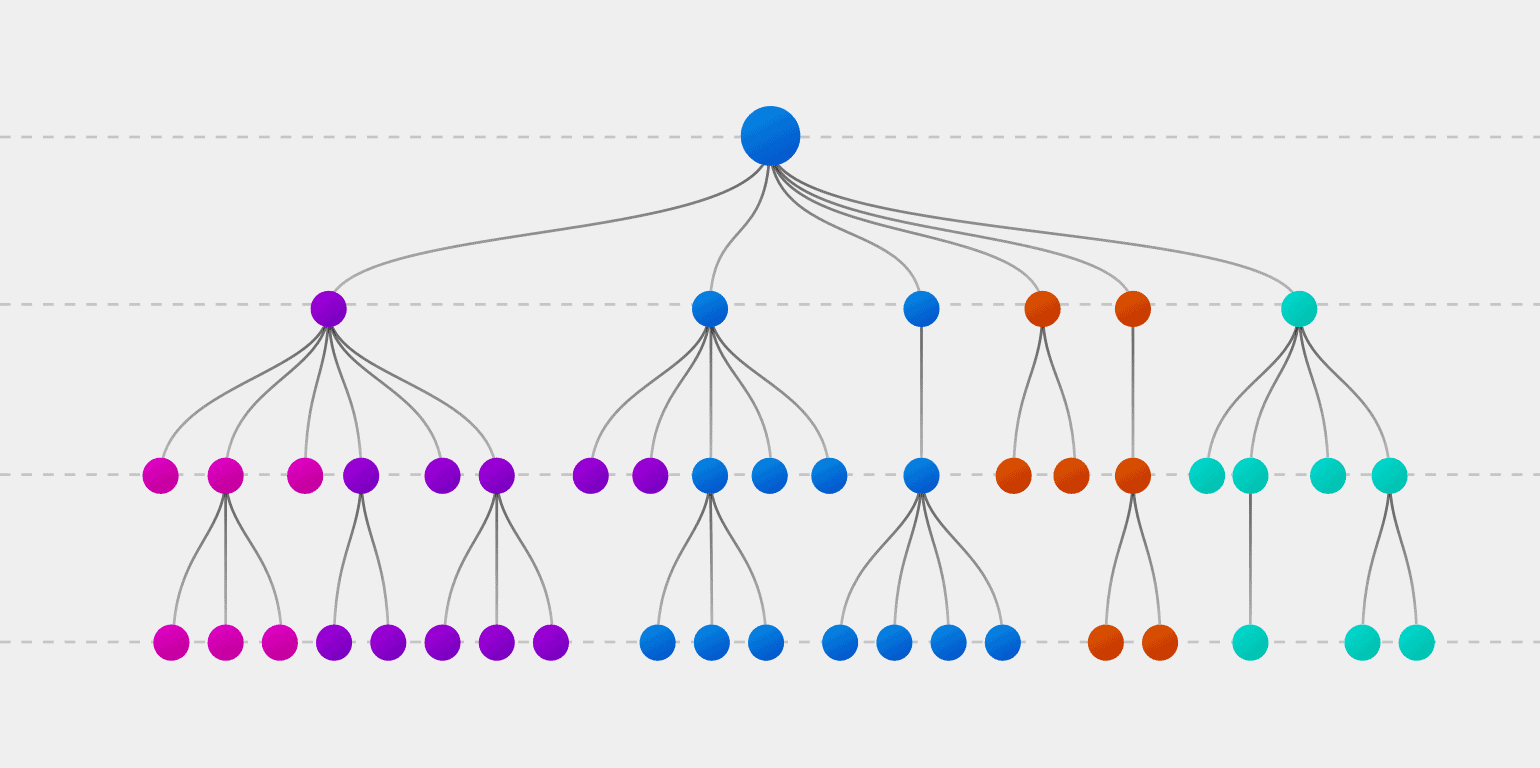
\includegraphics[width=12cm]{visuals/Decision-Trees-2.png}
    \caption{Decision Tree Visualization}
\end{figure}

\noindent
Decision Trees follow a tree structure where each node denotes a conditional statement on an attribute, each branch represents an outcome of the condition, and each leaf node holds a class label (call in or non call in). By aggregating the results of many decision trees, the random forest classifier prevents overfitting and errors due to biases.

\newpage
\subsection{Prediction Results}

The first evaluation metric I used was the area under the Receiver Operating Curve (ROC). The ROC Curve shows the trade-offs between the True Positive Rate (TPR) and the False Positive Rate (FPR). The higher the area under the ROC Curve, the better the model is at distinguishing between call-ins and non call-ins.
\\ \\
The area under the ROC curve using the RF Model was 0.79 which shows that the model does a decent job in distinguishing the two data classes. An area of 0.5, denoted by the area under the red line in the graph below, indicates a random guess in which the classifier is unable to distinguish between call ins and non call ins. 

\begin{figure}[htp]
    \centering
    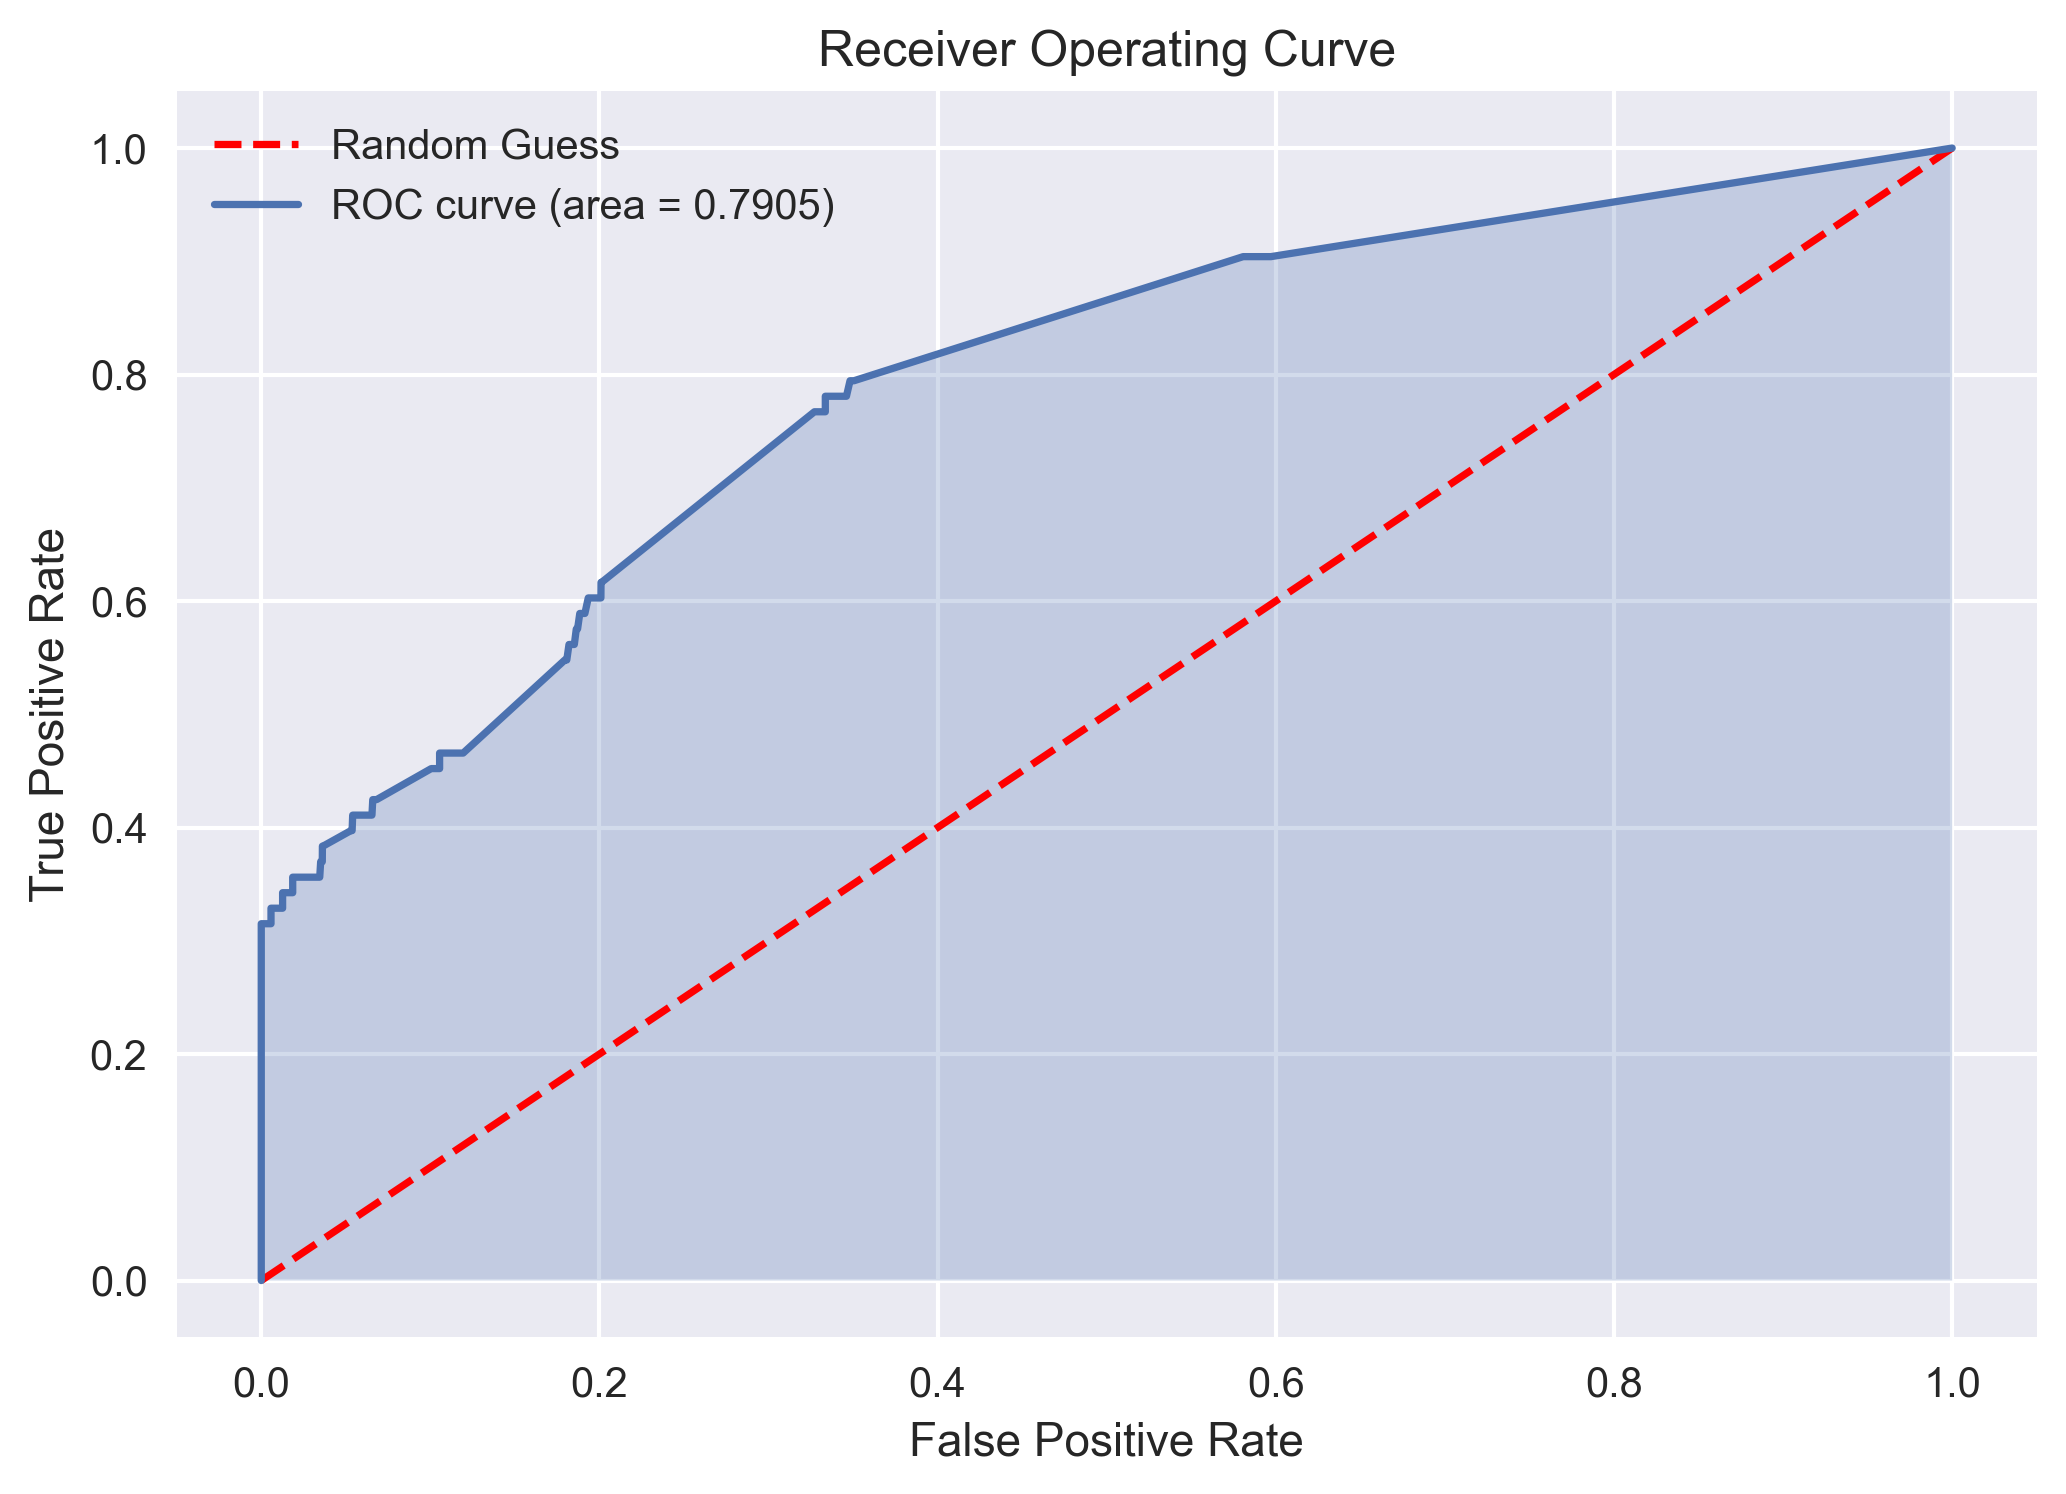
\includegraphics[width=12cm]{visuals/roc.png}
    \caption{ROC Curve}
\end{figure}

\newpage

\noindent
Apart from the ROC Curve, I used Accuracy, Recall, Precision, and the F1 Score to evaluate the Random Forest Classifier. After filtering the data set for outliers, the model's success drastically improved.

\begin{figure}[htp]
    \centering
    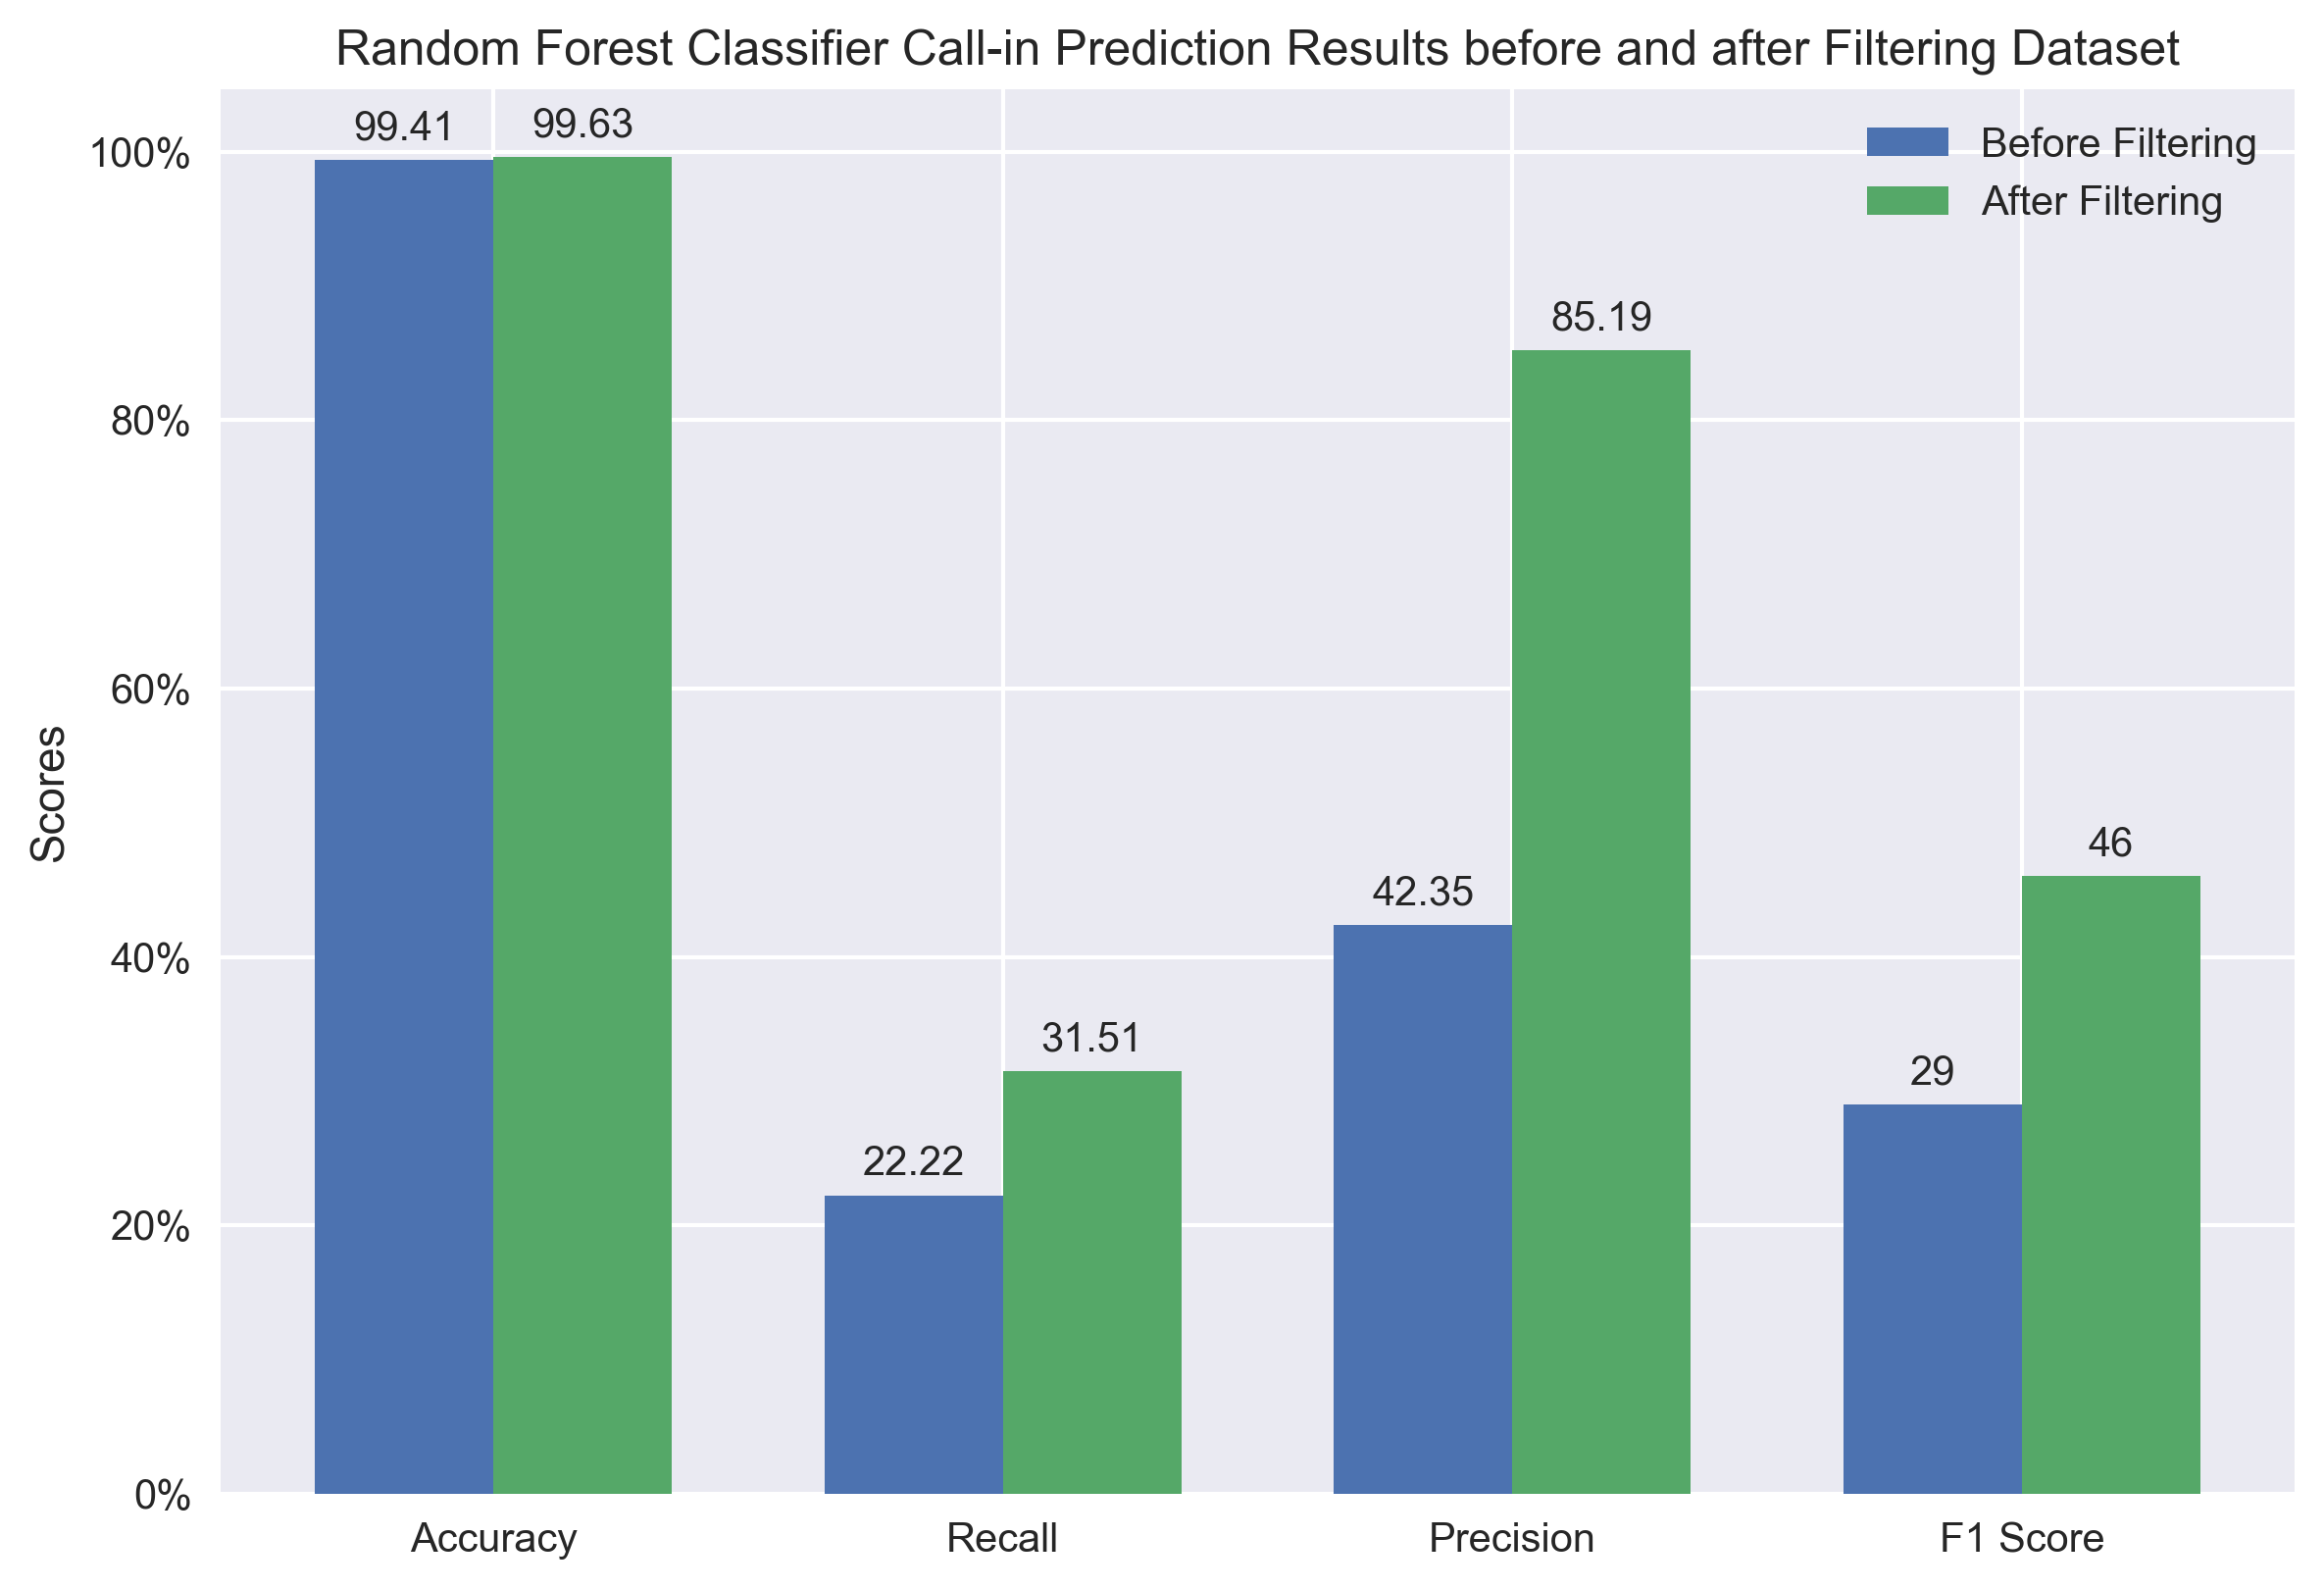
\includegraphics[width=12cm]{visuals/results_call-in.png}
    \caption{Random Forest Classifier Results}
\end{figure}

\noindent
As expected, the accuracy of the RF Classifier before and after filtering are extremely high because of the data imbalance. However, after filtering, the precision and recall increase significantly which shows the importance of ensuring that data is thoroughly processed before use. Finally, the F1 Score combines the precision and recall of a classifier into a single metric by calculating their harmonic mean: 

\begin{equation*}
    F_{1} = 2\times \frac{\text{Precision} \times \text{Recall}}{\text{Precision} + \text{Recall}}
\end{equation*}

\begin{equation*}
    \text{Precision} = \frac{\text{True Positives}}{\text{True Positives} + \text{False Positives}}
    ;
    \text{Recall} = \frac{\text{True Positives}}{\text{True Positives} + \text{False Negatives}}
\end{equation*}


\begin{figure}[htp]
    \centering
    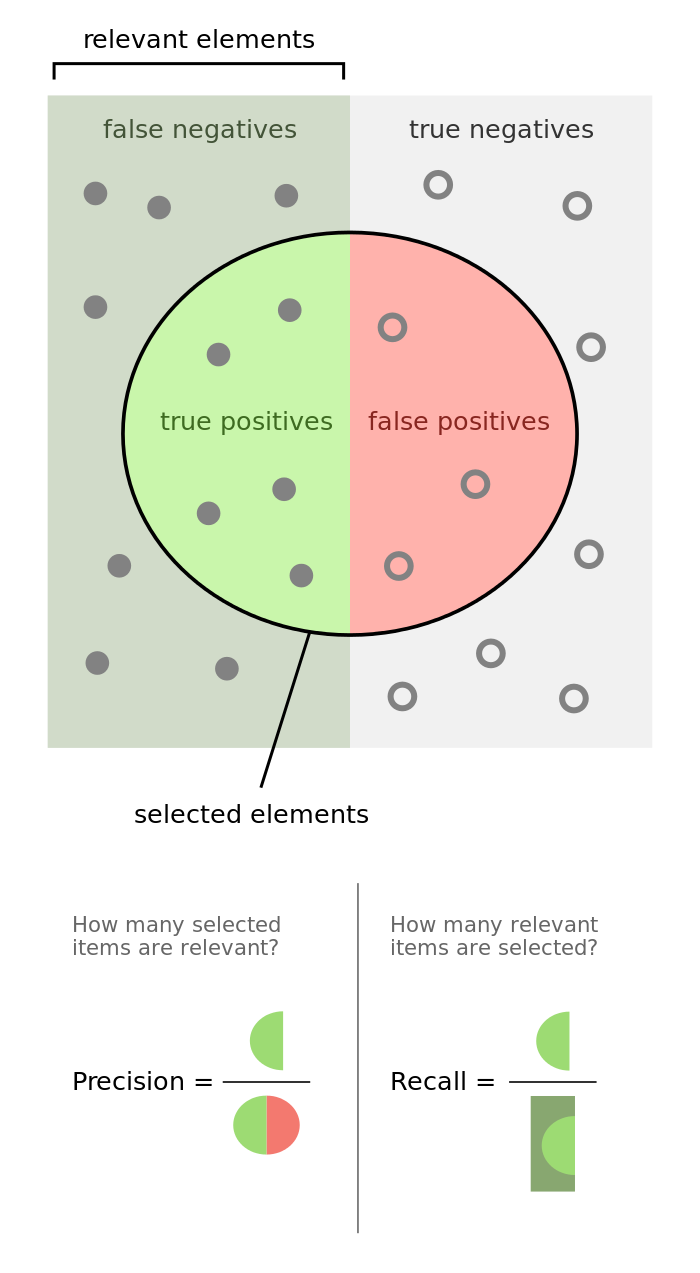
\includegraphics[width=10cm]{visuals/precisionrecall.png}
    \caption{Visualization of Precision and Recall}
\end{figure}

\newpage

\section{Lan Mac Addresses Data Analysis}

The next task I worked on was analyzing and correlating the lan macs data and the manufacturer mac addresses data:

\begin{enumerate}
    \item Lan Macs Data: Contains a Serial Number for all devices as well as a 'visible lan macs' column containing an list of mac addresses for each AP. 
    \item Manufacturer Mac Addresses Data: Includes the MAC address OUI list of manufactures and the prefix for each range of addresses. It describes each mac address range and the corresponding company that owns it.
\end{enumerate}
Using the two data sets and provided serial number, I determined how many mac addresses each company owns and added a 'manufacture list' column.

\begin{figure}[htp]
    \centering
    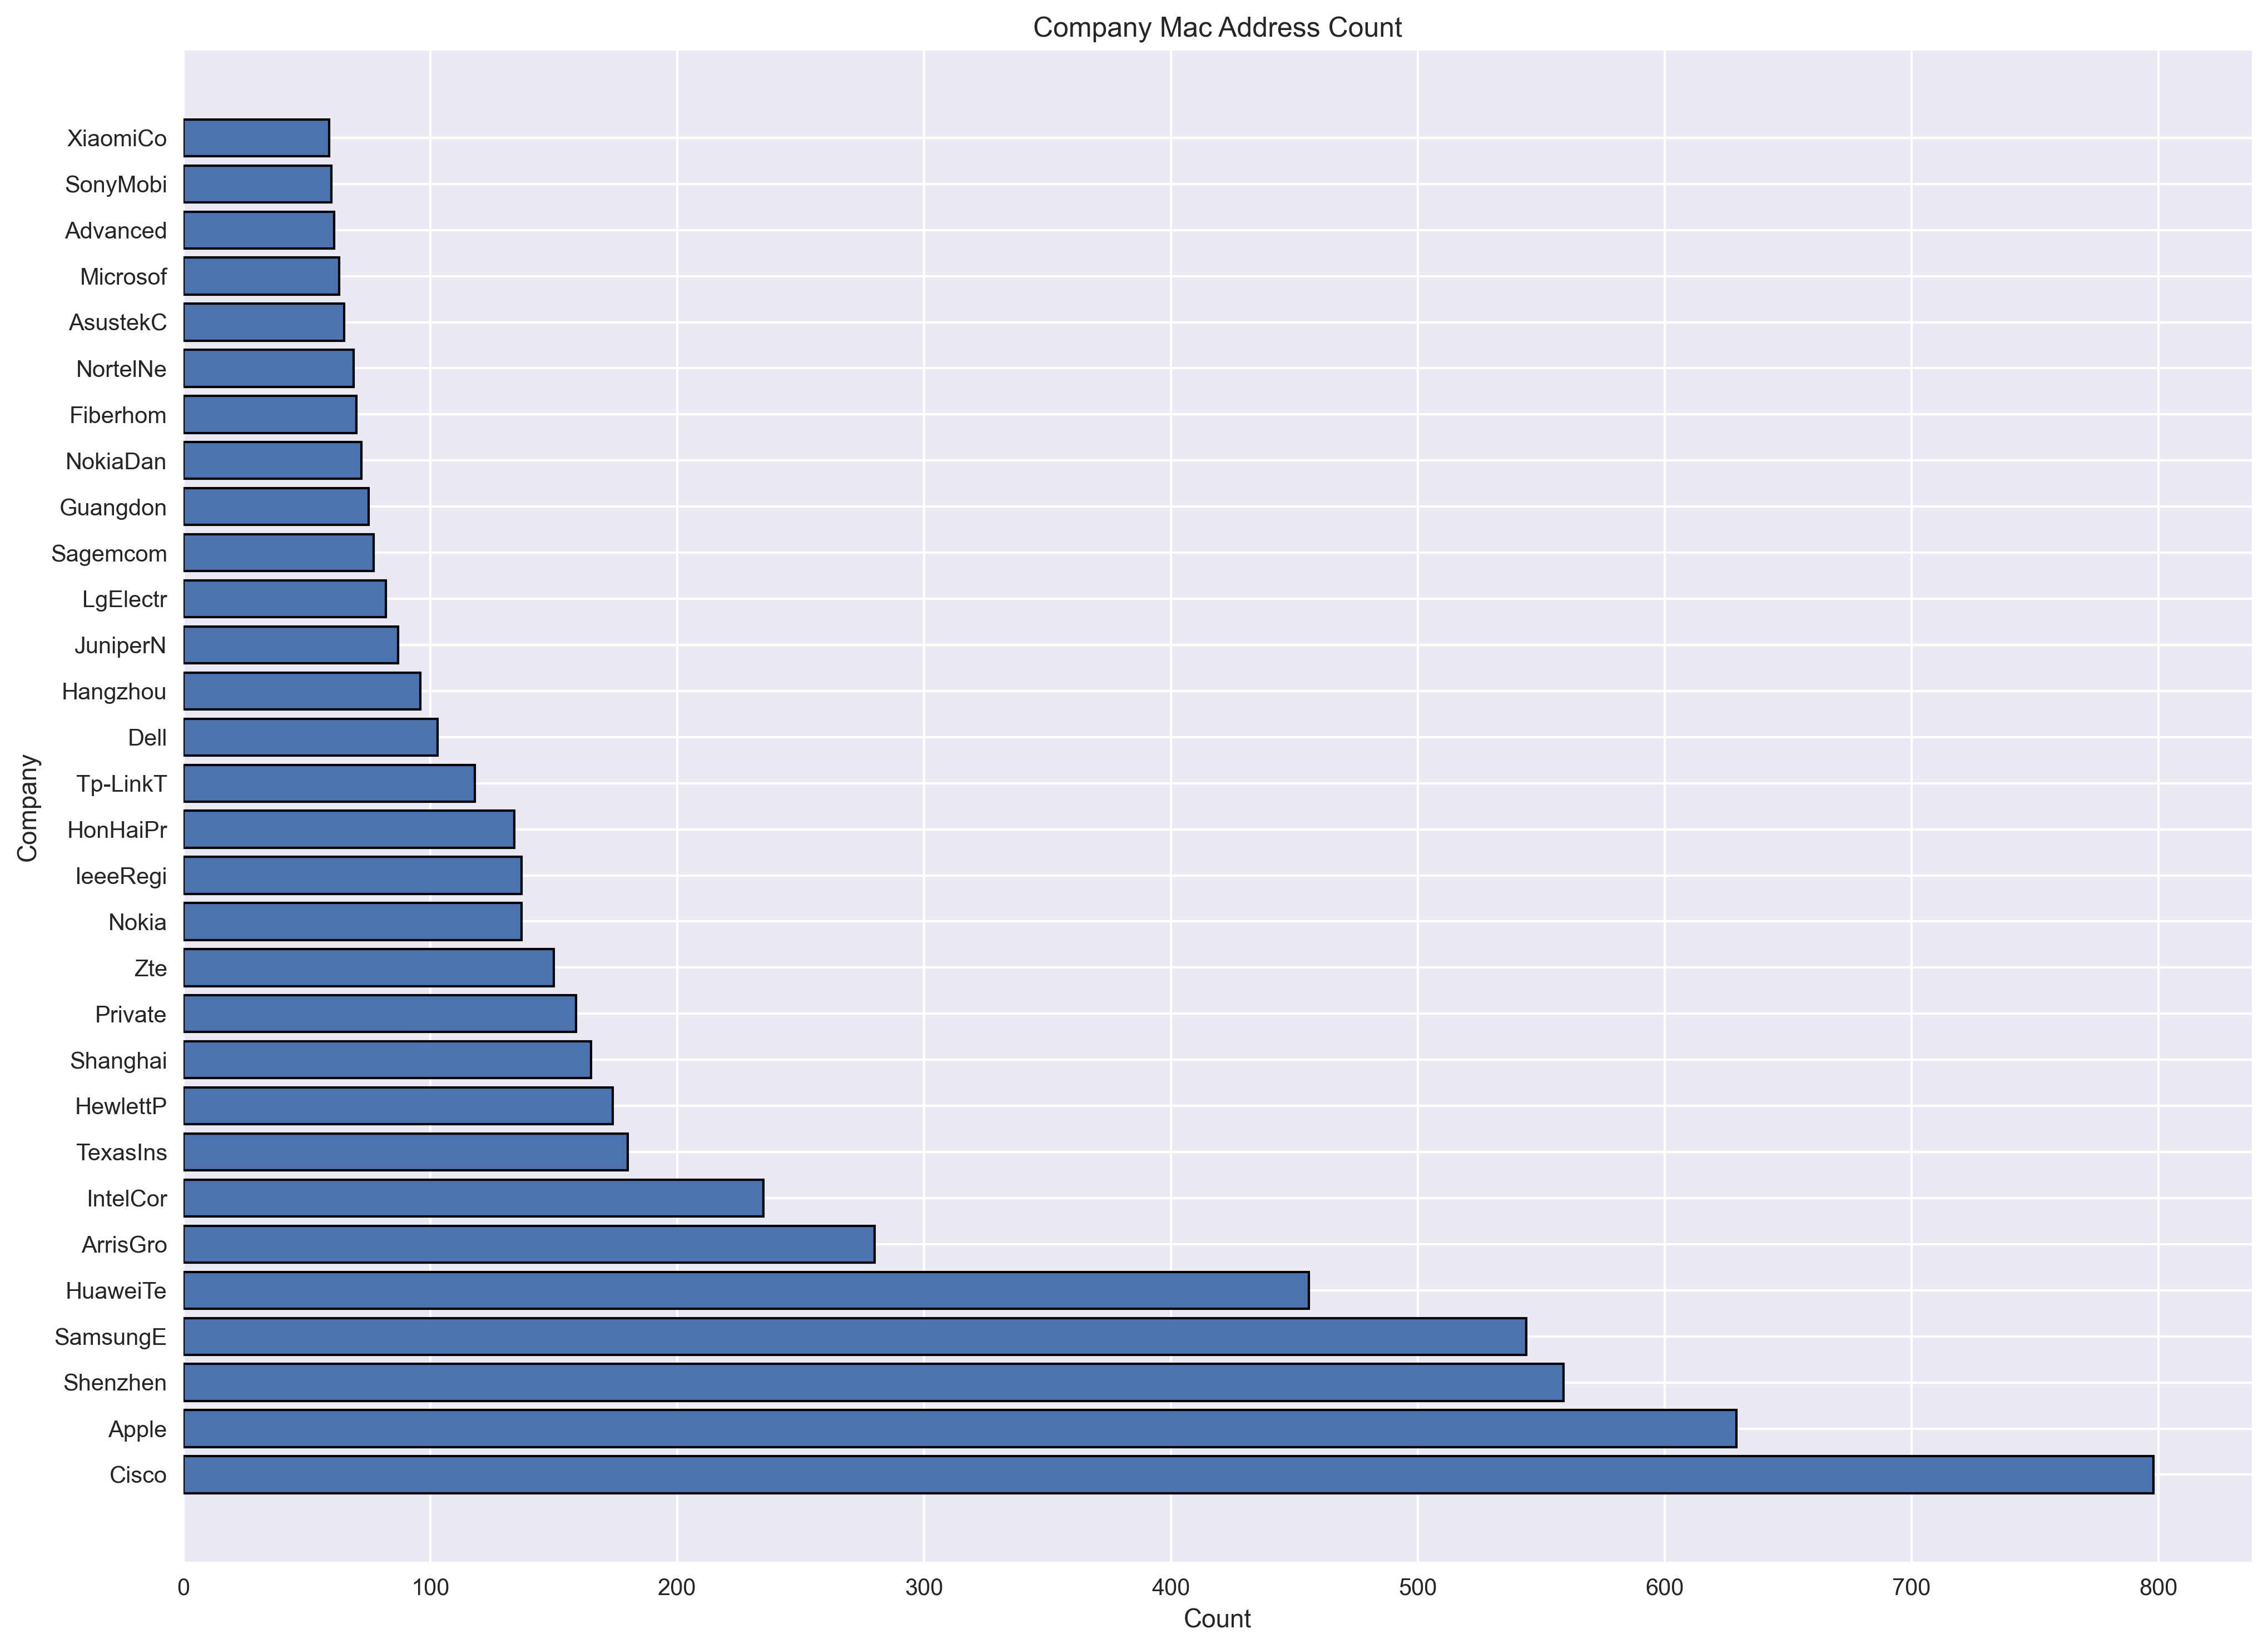
\includegraphics[width=12cm]{visuals/company_mac_address_counts.png}
    \caption{Random Forest Classifier Results}
\end{figure}

\begin{figure}[htp]
    \centering
    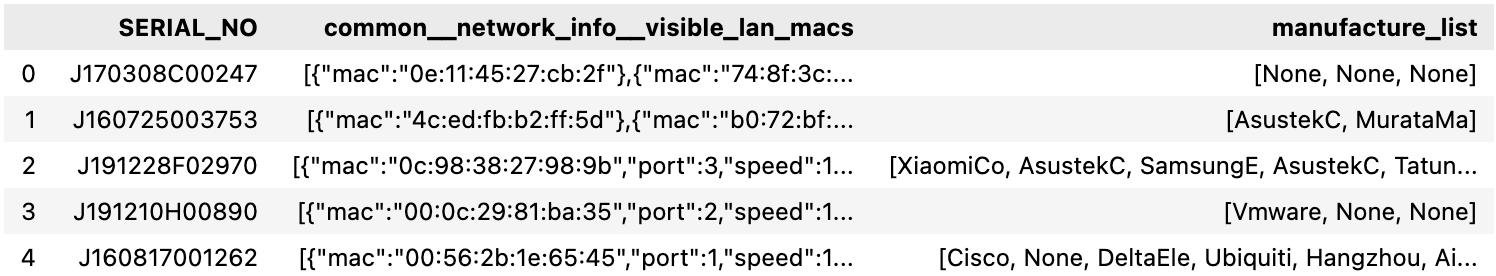
\includegraphics[width=10cm]{visuals/Screen Shot 2021-08-13 at 12.37.03 AM.png}
    \caption{Updated Lan Macs with Manufacture List}
\end{figure}

\newpage

\section{K-Means Clustering - Unsupervised Learning}

The final task I worked on was implementing PySpark's Clustering Algorithm on both the neighbors data and the previous AP - WiFi data.

\subsection{Neighbors Data Clustering}

Before applying the Clustering Algorithm, I had to combine the 2 neighbors data sets: 2.4 GHz Neighbors Data and 5 GHz Neighbors Data. Both data sets contain a neighbors feature which describes a list of neighbors for each device. Using this feature, I calculated the length of each neighbors array to create the 'neighbor counts' column, representing the number of neighbors for each device.   
\\ \\
For K-Means Clustering to be effective, it is essential that the data:
\begin{itemize}
  \item Only consists of numerical data as K-means uses distance measurements to classify data points into clusters. 
  \item Has no outliers or extreme skew. 
  \item Does not have a high level of correlation between any two features. 
\end{itemize}
Therefore, I created a correlation matrix to ensure that none of the features were highly correlated with each other:

\begin{figure}[htp]
    \centering
    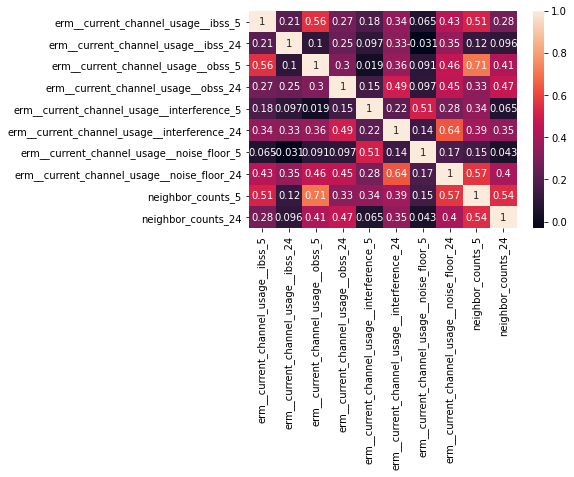
\includegraphics[width=10cm]{visuals/neighbors_correlation.png}
    \caption{Neighbors Correlation Matrix}
\end{figure}

\noindent
Before applying the K-means Clustering Algorithm, I had to determine the optimal number of clusters for the model to partition the data into. To determine the optimal k value, I calculated the silhouette scores for every clustering model with the k value in the range [2, 9]. The silhouette score of a clustering model ranges from 0 to 1. This metric is used to quantify how effective a model is in separating the data into different clusters. Therefore, a higher silhouette scores represents a greater separation. 

\begin{figure}[htp]
    \centering
    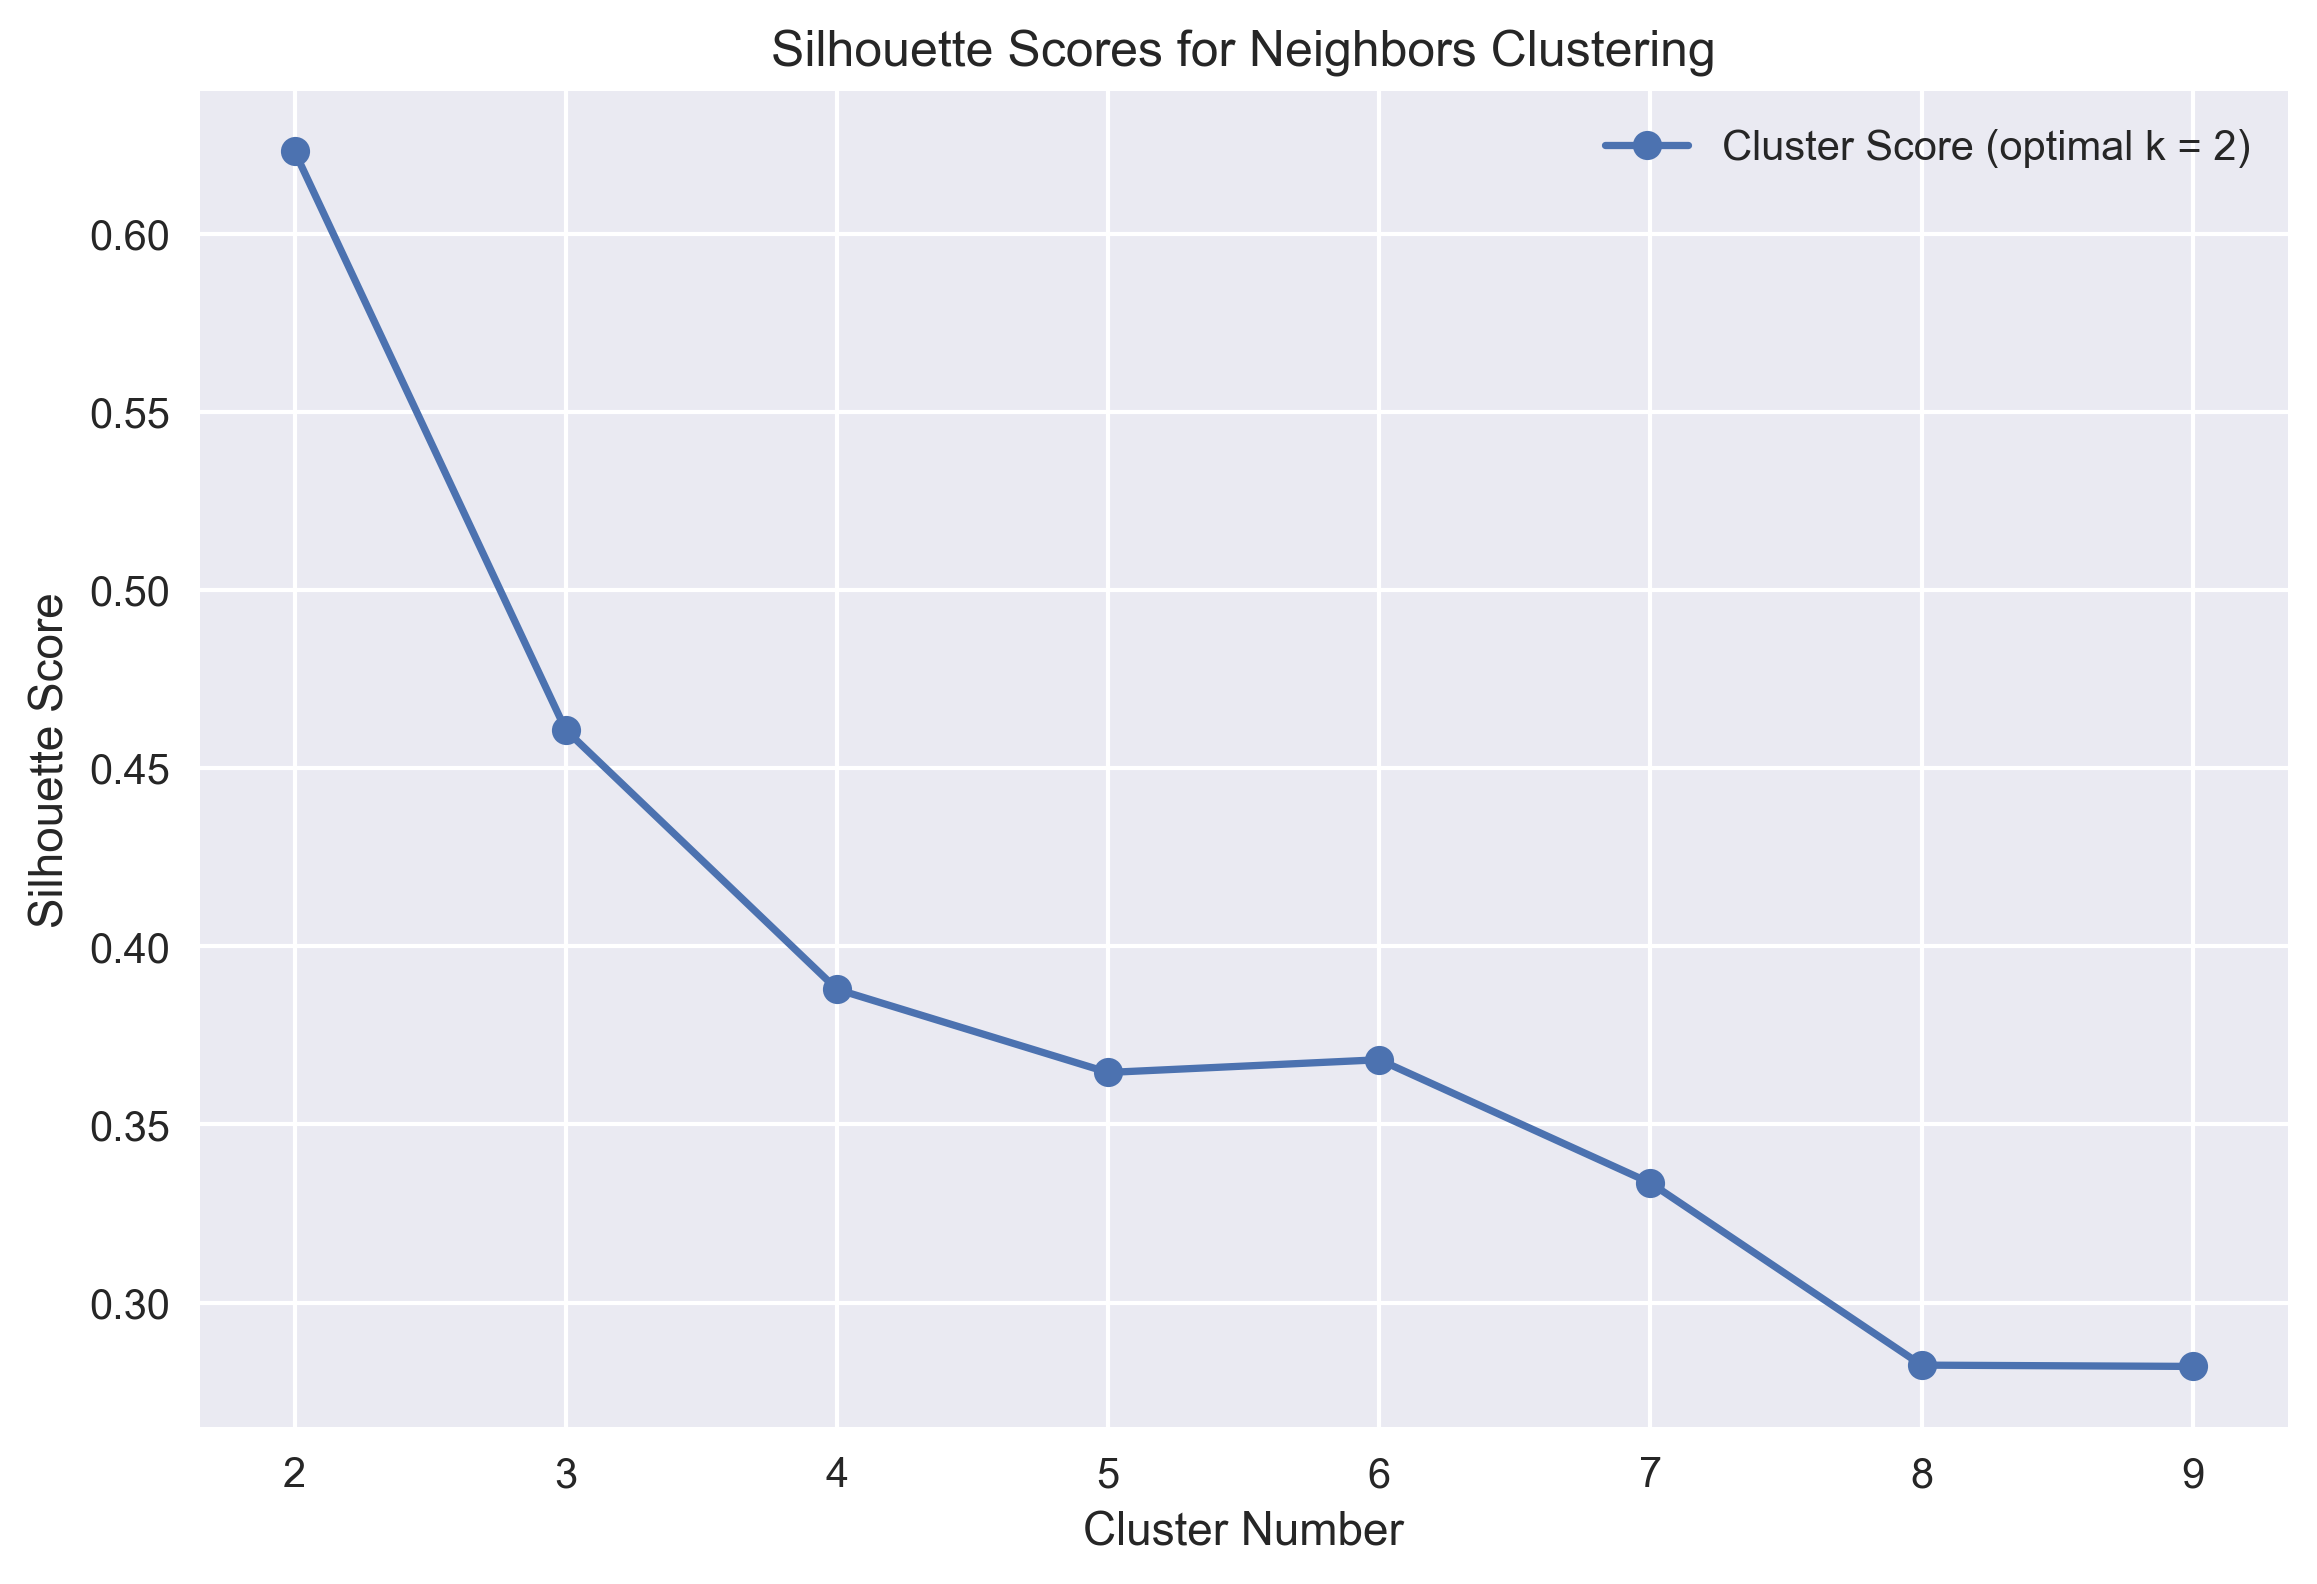
\includegraphics[width=12cm]{visuals/silhouette_scores_neighbors.png}
    \caption{Neighbors Silhouette Scores}
\end{figure}

\noindent
Plotting the silhouette scores against each other shows that the cluster of size 2 is the optimal number as it provides the highest separation. After k = 2, there is a downwards trend as increasing the number of clusters decreases the silhouette score.

\newpage
\noindent
Using k = 2, I used the K-Means Clustering Algorithm on the combined neighbors data set to get the following results:

\begin{figure}[htp]
    \centering
    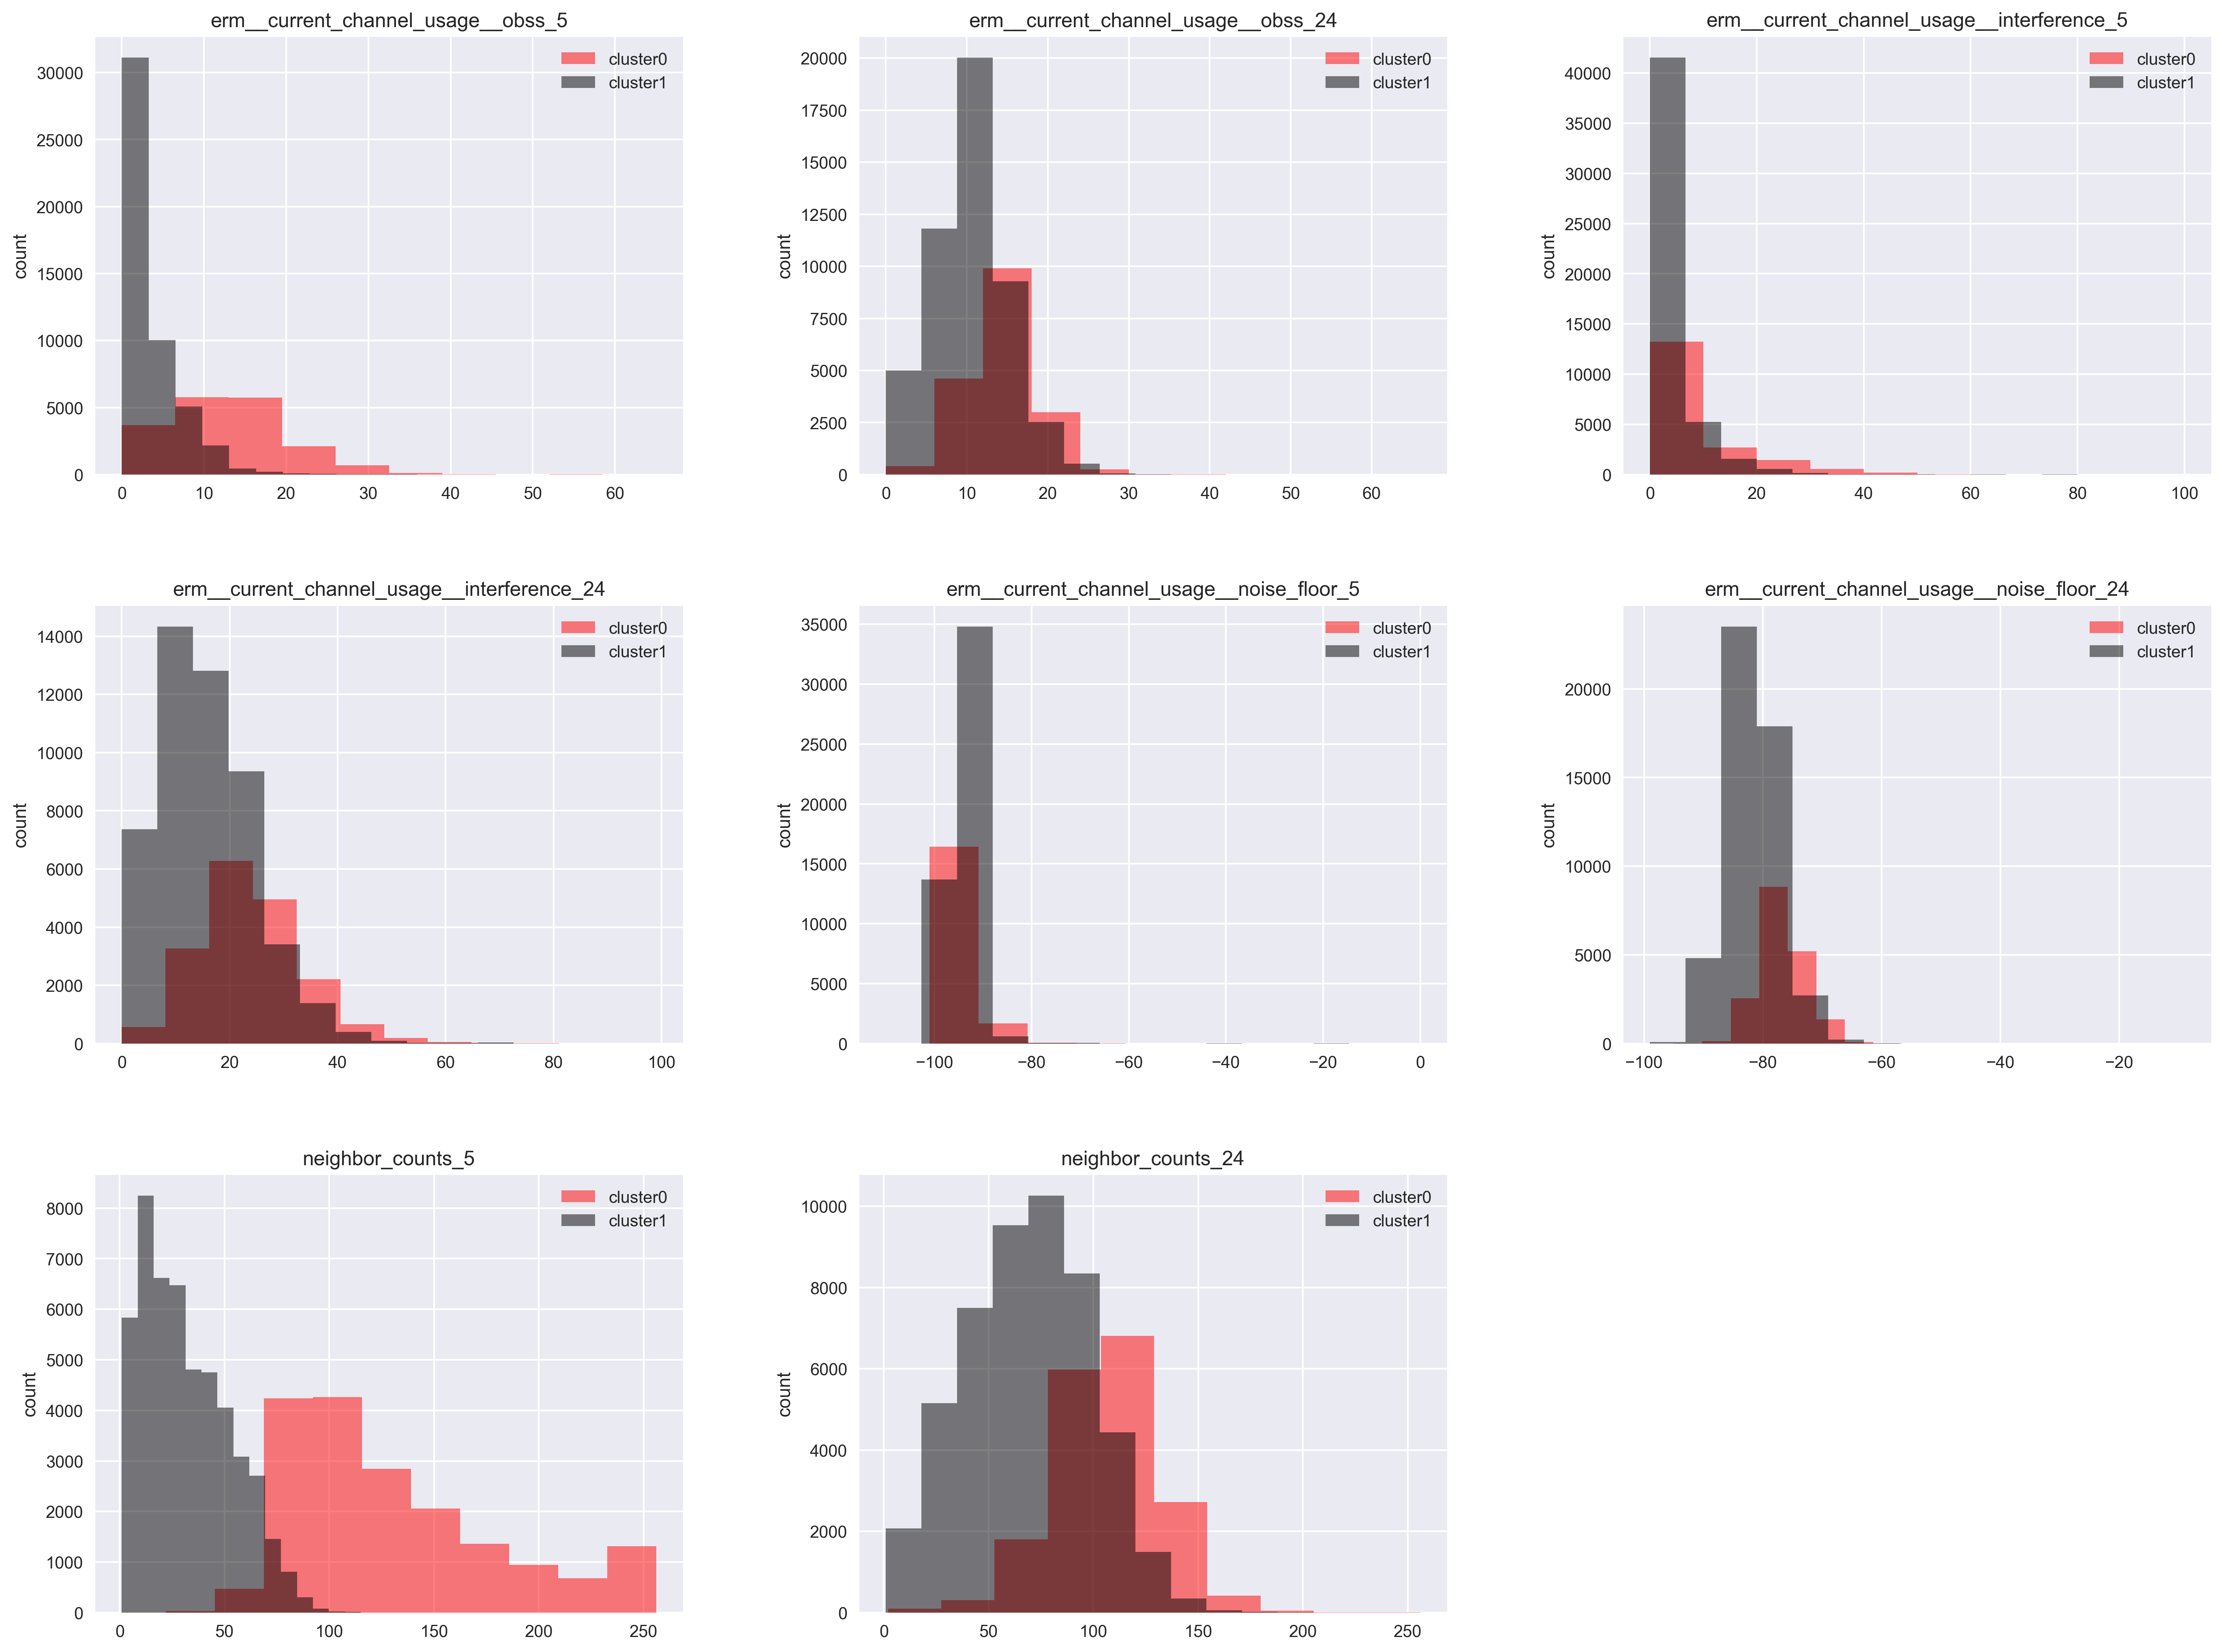
\includegraphics[width=14cm]{visuals/neighbors (2 clusters).png}
    \caption{Neighbors 2 Cluster Distribution}
\end{figure}

\noindent
Out of all the features, the neighbor counts (5 GHz) is the most prominent as it clearly shows the separation between the 2 clusters. Other promising features are the obss (5 GHz) and the neighbor counts (2.4 GHz). Using these results, it is possible to classify the data into high density and low density which can be used to explain and predict support call ins. 
\newpage
\noindent
After performing the initial clustering, I decided to analyze the size of each cluster as the graphs indicate that Cluster 0 (black) is significantly larger than Cluster 1 (red). After performing the clustering algorithms with k = 2 separately on the 2.4 GHz data and the 5 GHz data, I had 4 different clusters:

\begin{enumerate}[label=(\alph*)]
    \item Cluster 0 - 5 GHz
    \item Cluster 1 - 5 GHz
    \item Cluster 0 - 2.4 GHz
    \item Cluster 1 - 2.4 GHz
\end{enumerate}

\begin{figure}[htp]
    \centering
    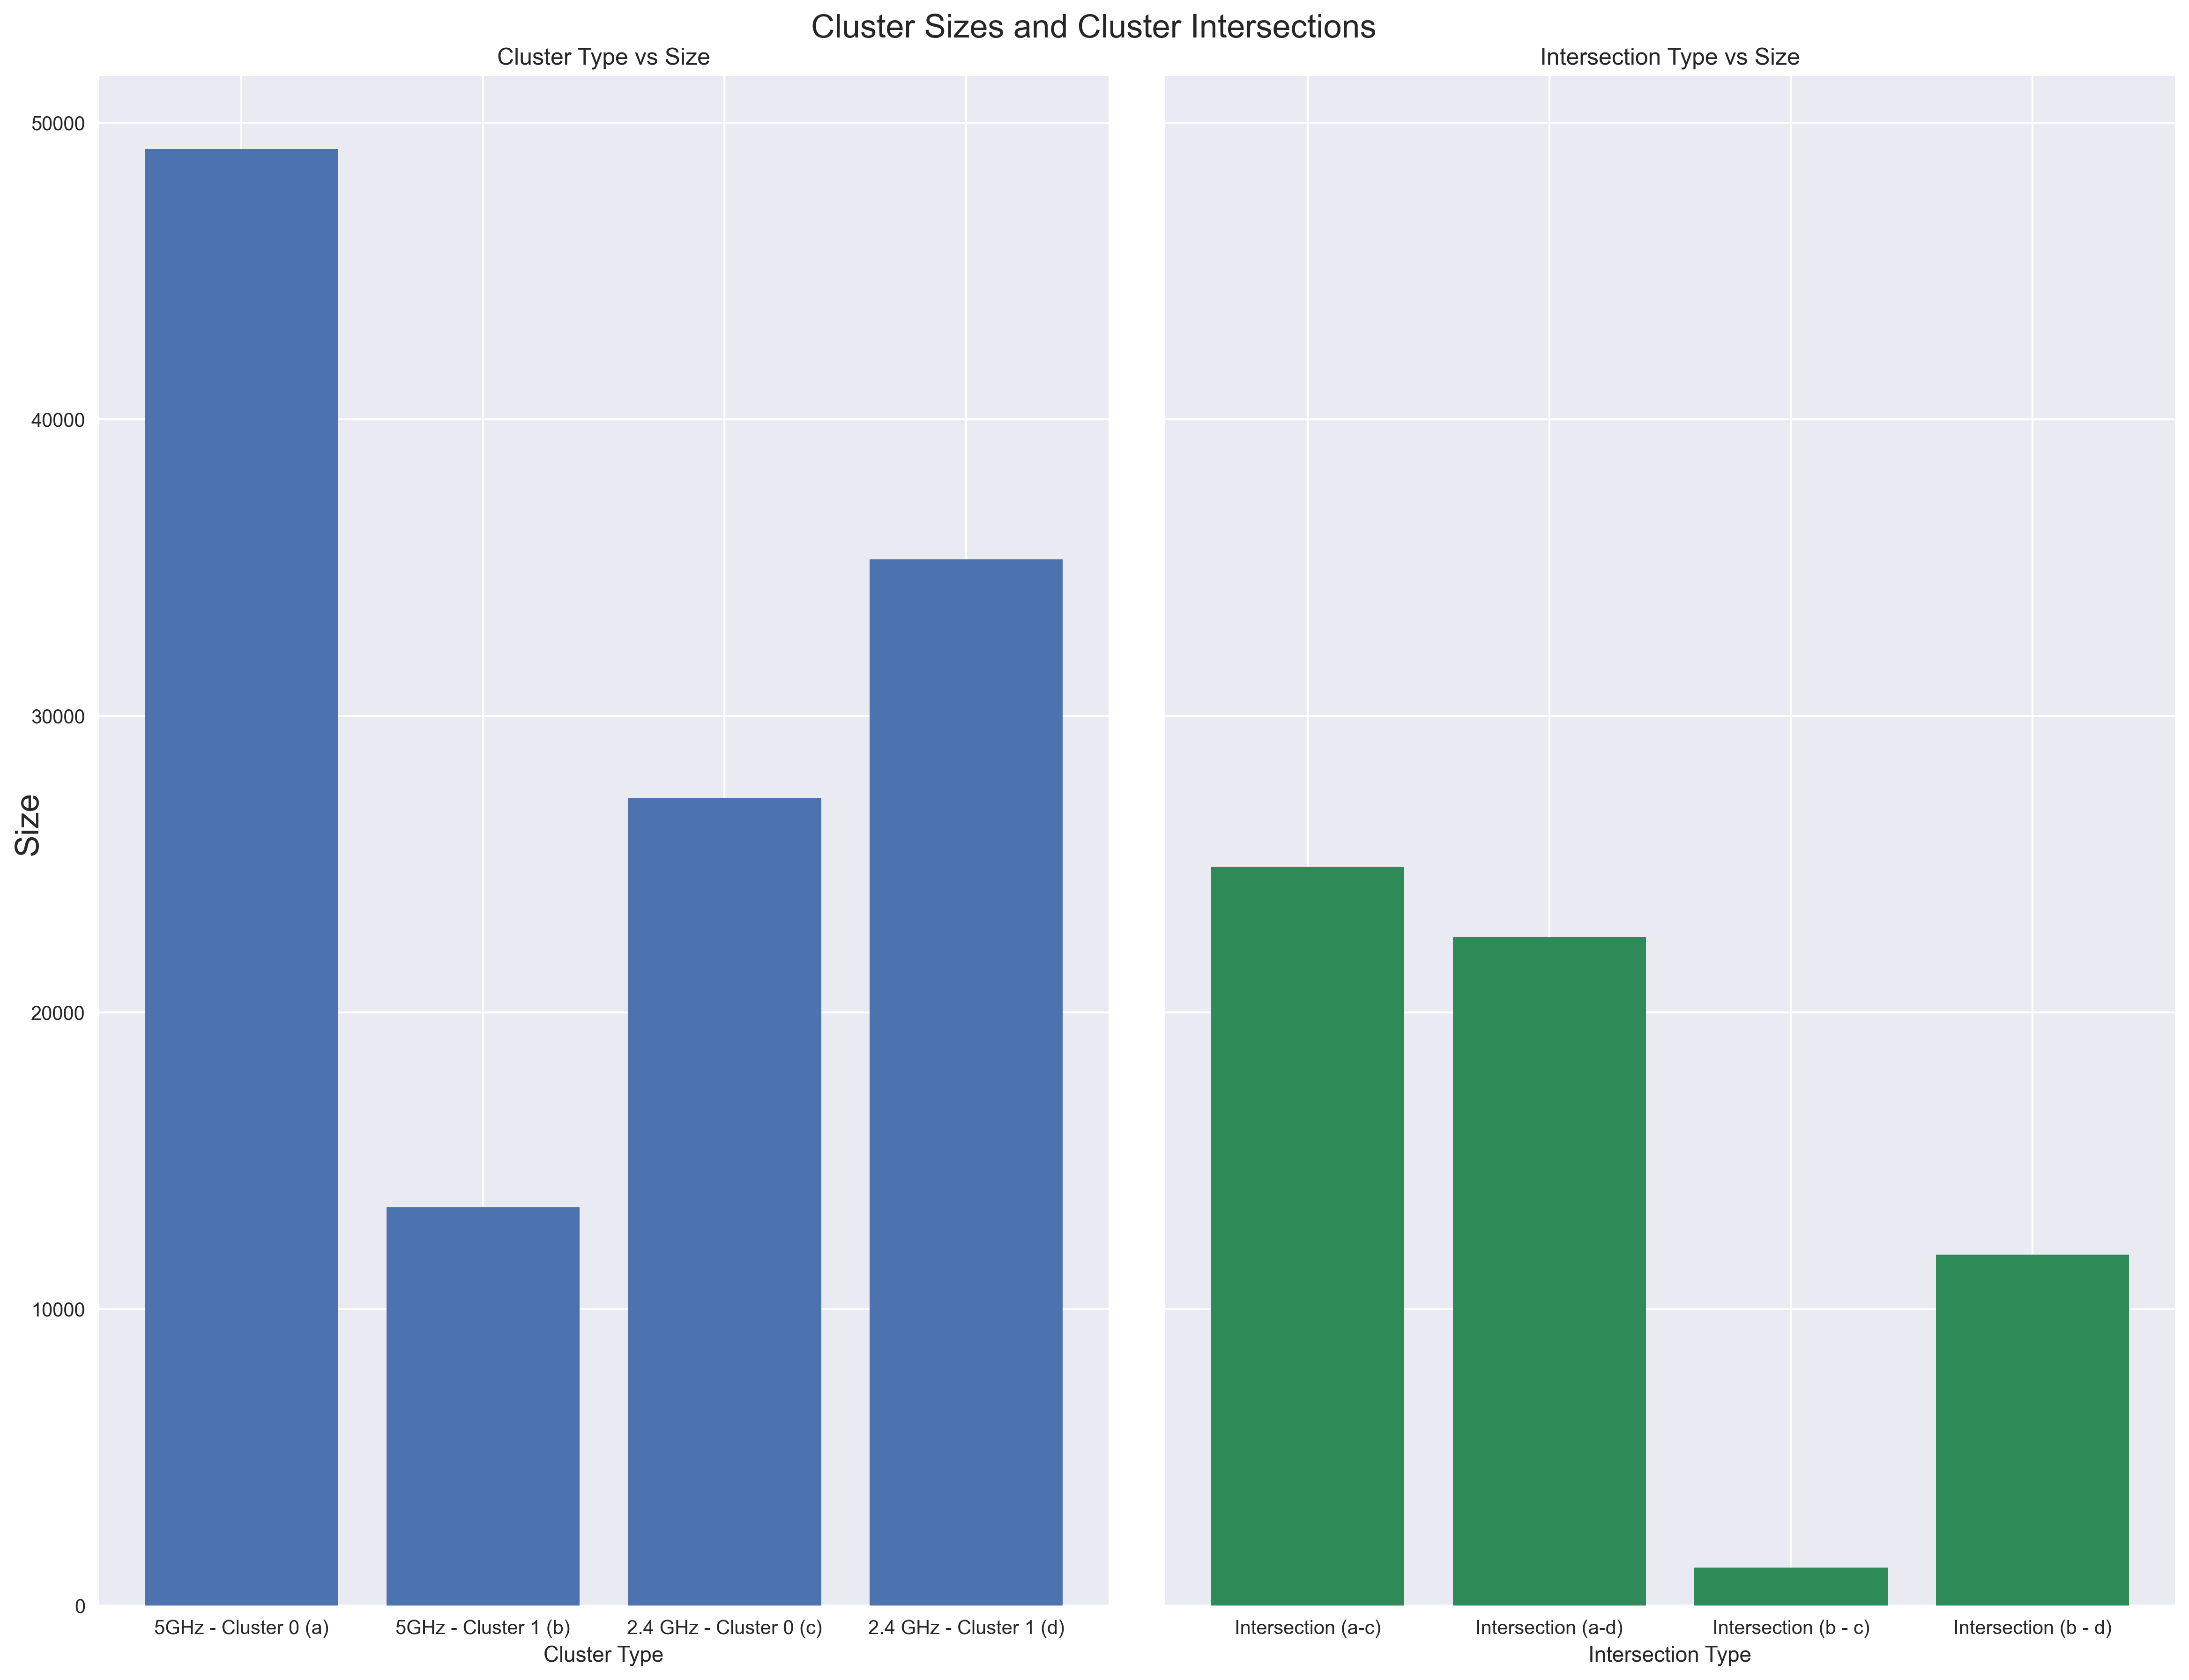
\includegraphics[width=14cm]{visuals/cluster_sizes_intersections.png}
    \caption{Cluster Sizes and Intersections}
\end{figure}

\noindent
The graph on the left shows the sizes of each cluster with the largest being Cluster 0 (5GHz) and the smallest being Cluster 1 (5 GHz). The graph on the right shows the sizes of intersections between the 2.4 GHz clusters and the 5 GHz clusters. The intersection size between clusters (b) and (c) is significantly smaller than the rest which suggests that 3 clusters might be more appropriate. Additionally, considering that the silhouette score for 3 clusters was the second highest score, I performed the K-Means algorithm with k = 3. The distribution of the 3 clusters for each feature in the combined neighbors data set is displayed below:

\begin{figure}[htp]
    \centering
    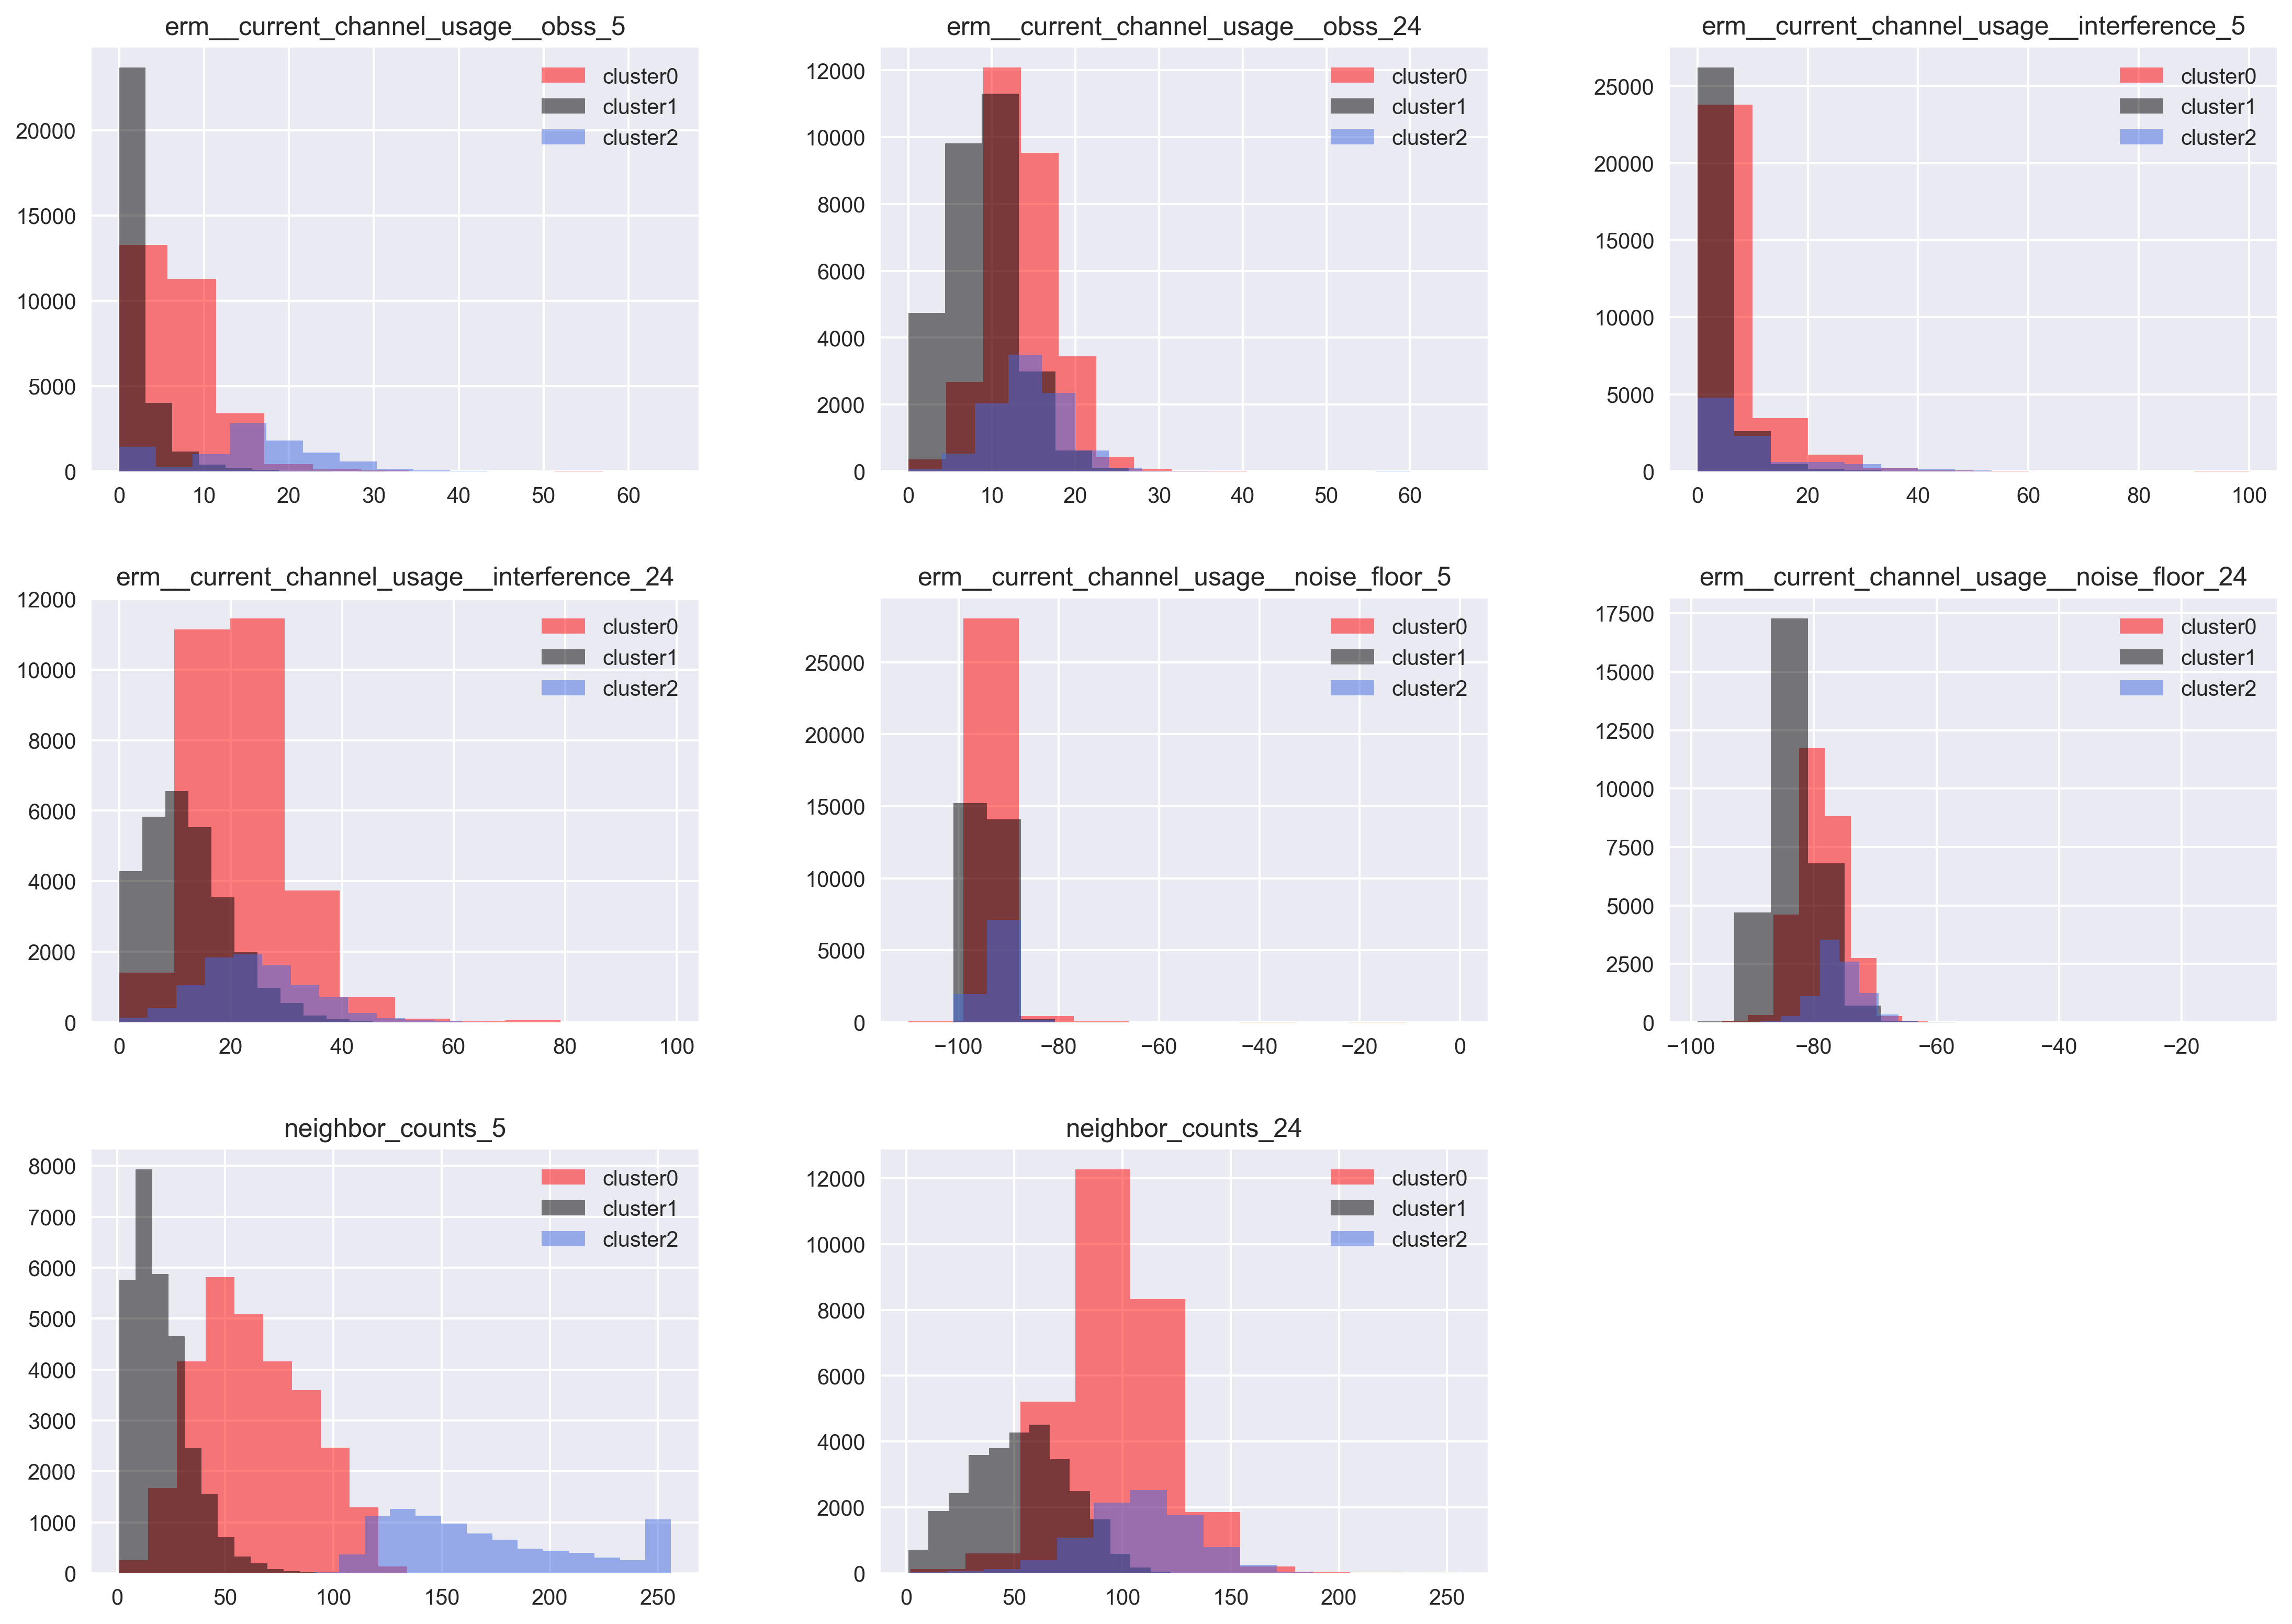
\includegraphics[width=14cm]{visuals/neighbors (3 clusters).png}
    \caption{Neighbors 3 Cluster Distribution}
\end{figure}

\noindent
Once again, the neighbor counts (5 GHz) is the most prominent feature as it distinctly shows the separation among the 3 clusters. Additionally, the obss (5 GHz), interference (2.4 GHz), and the neighbor counts (2.4 GHz) are important features to consider as they also show significant separation between the 3 clusters. By using 3 clusters instead of 2 clusters, it is possible to classify the data into urban, suburban, and rural which may be valuable for customers.


\newpage

\subsection{AP - WiFi Data Clustering}

In addition to applying the K-Means Clustering Algorithm on the neighbors data set, I revisited the initial AP - WiFi Data consisting of:

\begin{enumerate}
    \item AP Data: It contains a unique Serial Number for all devices (call in and non call in) and many numerical features describing the specific AP. 
    \item WiFi CIR Data: It contains categorical information for call-in devices such as the unique Serial Number, Device Type Name, and the AP Software Version
\end{enumerate}

\noindent
Before performing the clustering, I calculated the silhouette scores for k in the range [2, 9] to determine the optimal number of clusters that will result in the greatest separation. Graphing the silhouette scores reveals that the clustering model is the most successful at distinguishing between 2 clusters. In comparison to the Neighbors data set, the AP - WiFi silhouette scores are significantly higher across all k-values which suggests that the clustering algorithm is more appropriate for this data set as it has more features to choose from. 

\begin{figure}[htp]
    \centering
    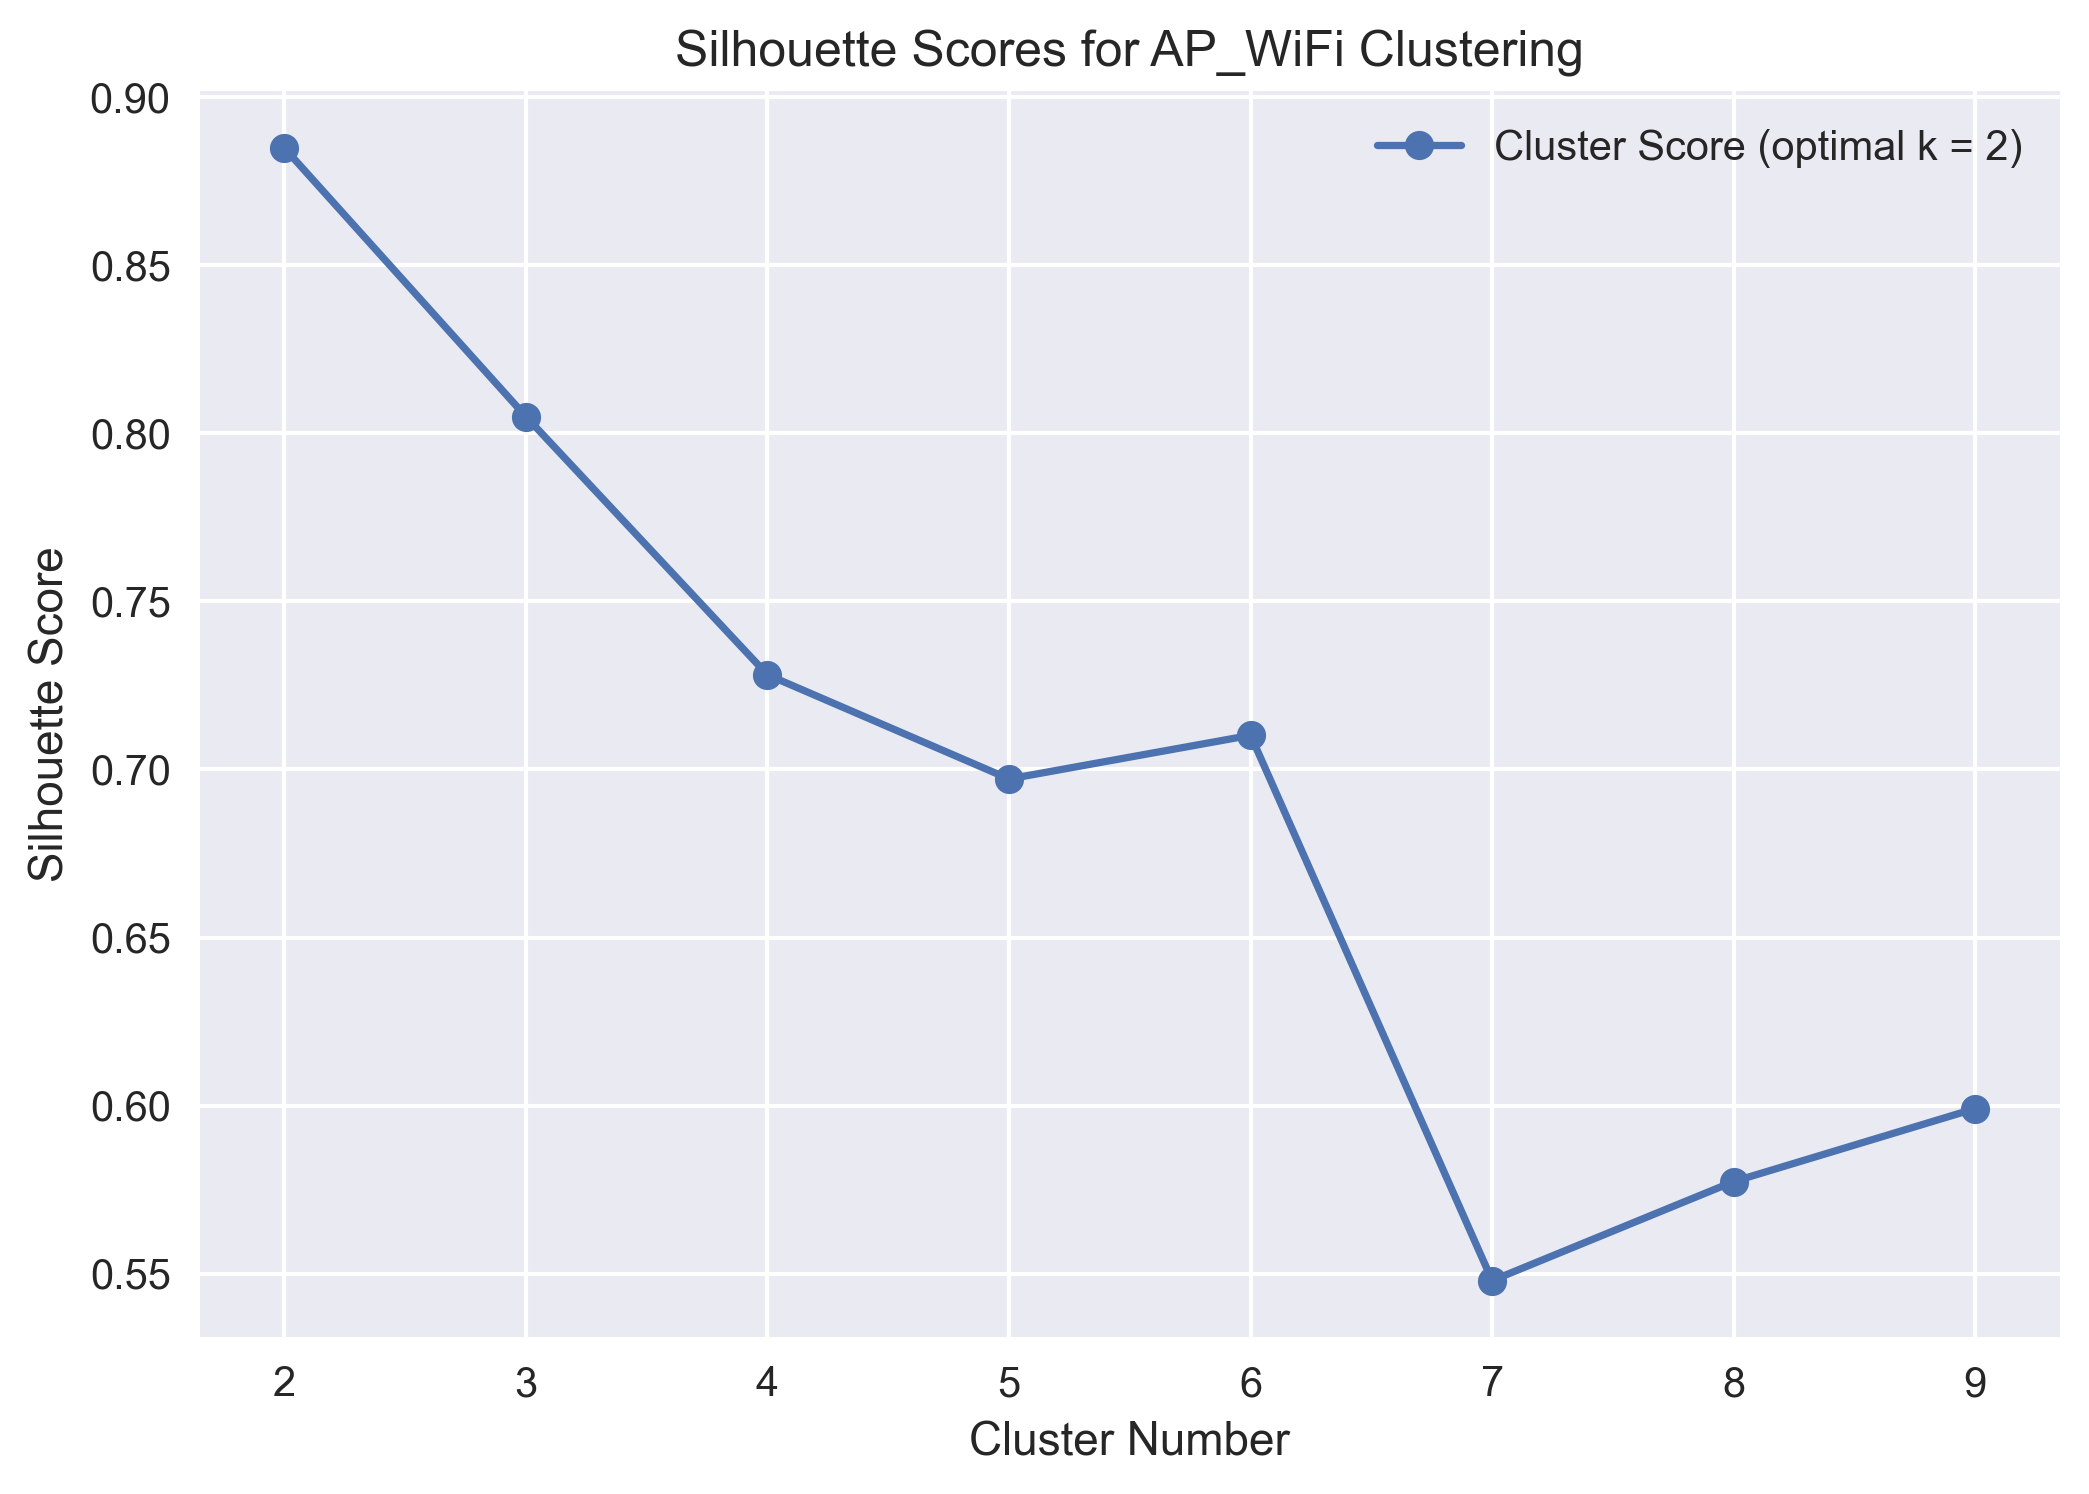
\includegraphics[width=12cm]{visuals/silhouette_scores_ap_wifi.png}
    \caption{AP - WiFi Silhouette Scores}
\end{figure}

\newpage
\noindent
Given the high silhouette score for 2 clusters, I applied the clustering model on the data in hopes that it would separate the call ins from the non call ins. Although the algorithms failed to completely separate the call ins, it did manage to group all the call ins in cluster 0 which is seen below: 

\begin{figure}[htp]
    \centering
    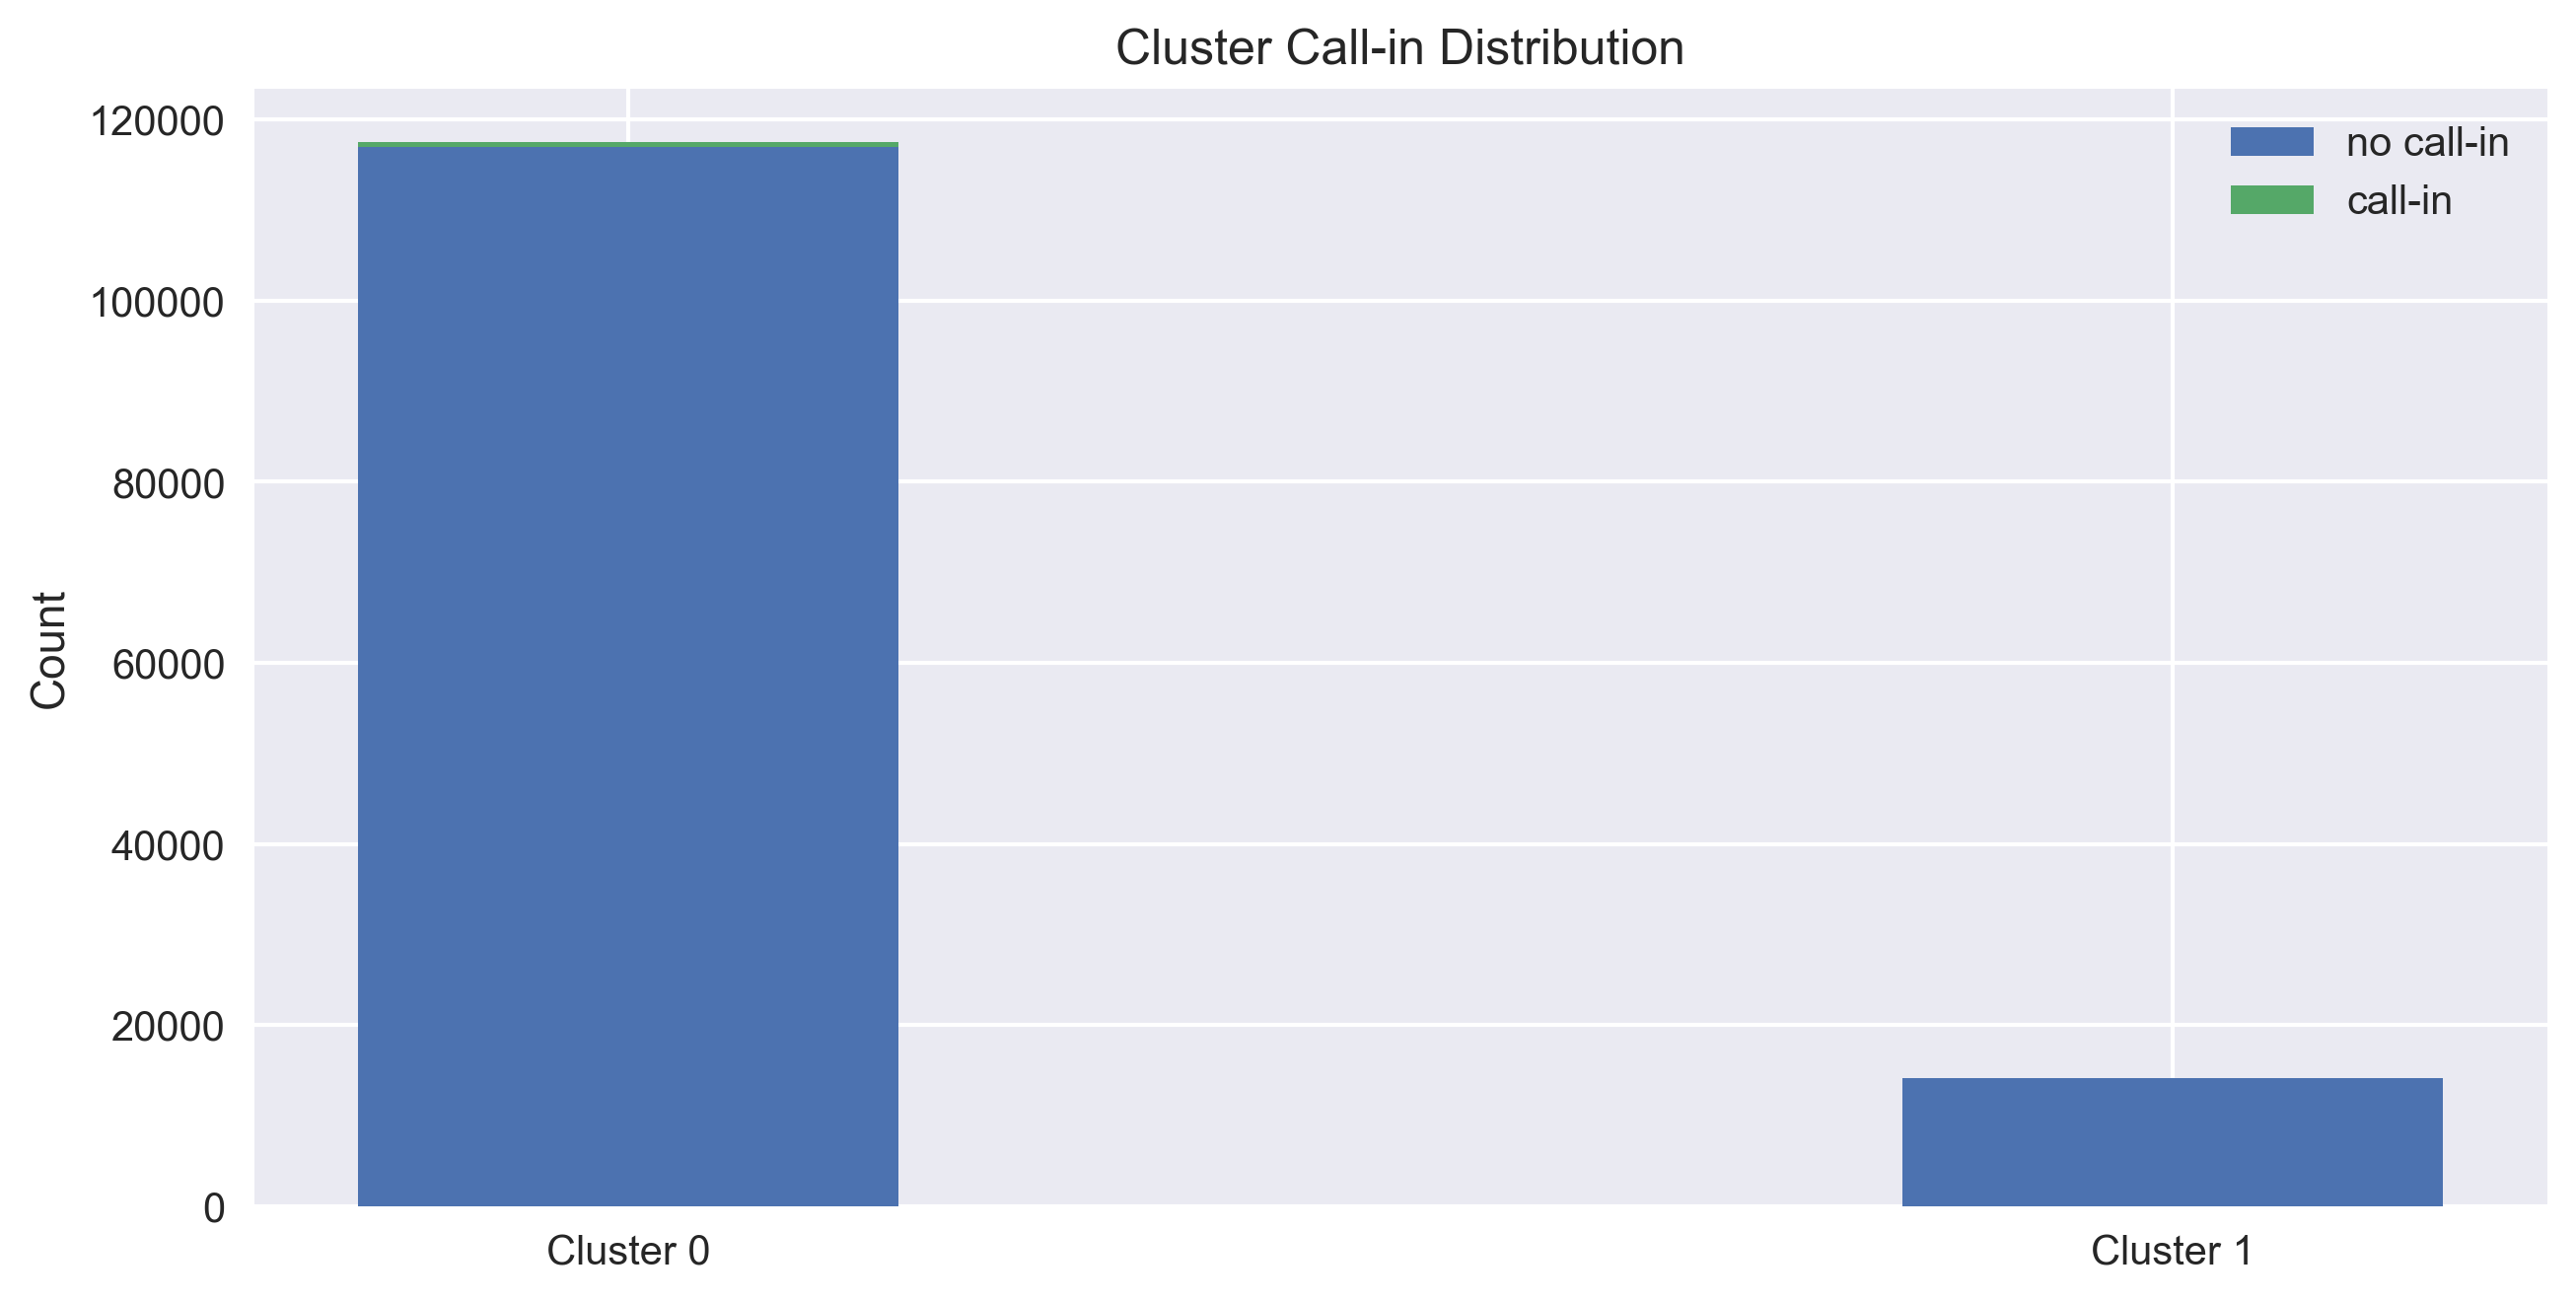
\includegraphics[width=12cm]{visuals/cluster_call-in_distribution.png}
    \caption{Cluster Call-in Skewed Distribution}
\end{figure}

\begin{center}
    \begin{tabular}{ |p{3cm}||p{3cm}|p{3cm}| }
        \hline
        \multicolumn{3}{|c|}{Distribution of call ins} \\
        \hline
        Cluster Number & Call-in Count & Non Call-in Count \\
        \hline
        0 & 531 & 116966\\
        1 & 0 & 14138\\
        \hline
    \end{tabular}
\end{center}

\noindent
\\
Despite the K-Means clustering algorithm failing to isolate all the call ins in its own cluster, the model managed to group all the call ins together in cluster 0, resulting in cluster 1 having 0 support call ins. This pattern suggests that the model was confident in classifying the data in Cluster 1 as non call ins. Therefore, this model can be used in the support call in prediction model as using the clustering model to confidently remove non call in devices will reduce the size of the data and the imbalance between call ins and non call ins.

\newpage
\section{Reflection}

Overall, I had a great time interning at embedUR this summer with the Data Mining/Machine Learning team. I am very grateful for this internship as it gave me the opportunity to refine my programming skills and apply powerful tools such as PySpark, Pandas, Matplotlib, and a variety of Machine Learning algorithms. Finally, I appreciate the amazing support of my mentors, John-Mark and Ben, for devoting their time to helping me overcome the many errors and doubts I encountered. They have instilled important coding practices for becoming a successful data scientist by stressing the importance of writing reusable code, providing many data visualizations, and ensuring that my code is clear and concise. 
\\ \\
One takeaways I have from this experience is the importance of supplementing my code with visuals that describe and enhance my results. Visualization is especially important when working with extremely large data sets that are incomprehensible just by looking at numbers. Using visualizations, data scientists and machine learning engineers can very quickly recognize patters in the data which is essential in trying to decipher the results of any Machine Learning algorithm. 
\\ \\
Another concept that I learned during the internship is the importance of writing reusable code. At first, I found myself writing the same code over and over again, especially when performing the clustering on the neighbors data and the AP - WiFi data. Additionally, if I found an error in one code segment, I would have to apply the same fixes in other places, making the risk of human error higher. Therefore, I decided to write general purpose Spark programs that I could re-use across the many code files I have. By only having to manage code in one location rather than across many files, I became more efficient and was able to avoid errors.
\lfoot{\href{https://sidnath.web.app/}{\underline{Personal Website}} | \href{https://github.com/SidNath21/embedur}{\underline{Access Code/Visuals}}}.  
\end{document}
